\documentclass[10pt,a4paper]{article}
\usepackage[T1]{fontenc}
\usepackage[utf8]{inputenc}
\usepackage{lmodern}
\usepackage{microtype}
\usepackage[margin=2.1cm,top=2.5cm,bottom=2.3cm]{geometry}
\usepackage{amsmath,amssymb,mathtools,bm}
\usepackage{booktabs,array,tabularx,multirow,longtable}
\usepackage[dvipsnames,table]{xcolor}
\usepackage{graphicx,float,caption,subcaption}
\usepackage{enumitem,titlesec,fancyhdr,fancyvrb}
\usepackage{tcolorbox}
\usepackage[colorlinks=true,linkcolor=ink,citecolor=ink,urlcolor=ink]{hyperref}

\definecolor{ink}{HTML}{1F4E79}
\definecolor{accent}{HTML}{2A9D6F}
\definecolor{amber}{HTML}{B26A00}
\definecolor{slate}{HTML}{5F6B7A}
\definecolor{paper}{HTML}{F4F7FB}

\setlength{\parskip}{0.55em}\setlength{\parindent}{0pt}
\renewcommand{\arraystretch}{1.18}
\setlist{itemsep=0.15em,topsep=0.3em,parsep=0pt}
\captionsetup{font=small,labelfont={bf,color=ink},labelsep=period,justification=raggedright,singlelinecheck=false,skip=4pt}
\setcounter{tocdepth}{1}

\titleformat{\section}{\Large\sffamily\bfseries\color{ink}}{\thesection}{0.7em}{}[\vspace{-0.4em}\textcolor{ink!35}{\titlerule[0.8pt]}]
\titleformat{\subsection}{\large\sffamily\bfseries\color{ink}}{\thesubsection}{0.6em}{}
\titleformat{\subsubsection}{\normalsize\sffamily\bfseries\color{slate}}{\thesubsubsection}{0.5em}{}
\titlespacing*{\section}{0pt}{1.8em}{0.8em}
\titlespacing*{\subsection}{0pt}{1.2em}{0.4em}

\pagestyle{fancy}\fancyhf{}
\fancyhead[L]{\small\sffamily\textcolor{slate}{Substrate Predictor}}
\fancyhead[R]{\small\sffamily\textcolor{slate}{Eton iGEM Dry Lab 2026}}
\fancyfoot[C]{\small\sffamily\textcolor{slate}{\thepage}}
\renewcommand{\headrulewidth}{0.3pt}\renewcommand{\headrule}{\hbox to\headwidth{\color{ink!30}\leaders\hrule height \headrulewidth\hfill}}

\newtcolorbox{keybox}[1][Key findings]{colback=paper,colframe=ink,coltitle=white,fonttitle=\sffamily\bfseries\small,title=#1,boxrule=0.6pt,arc=2pt,left=8pt,right=8pt,top=5pt,bottom=5pt,before skip=8pt,after skip=10pt}
\newtcolorbox{bionote}[1][Biology note for ML readers]{colback=accent!6,colframe=accent!80!black,coltitle=white,fonttitle=\sffamily\bfseries\small,title=#1,boxrule=0.6pt,arc=2pt,left=8pt,right=8pt,top=5pt,bottom=5pt,before skip=8pt,after skip=10pt}
\newtcolorbox{caveat}[1][Limitation]{colback=amber!7,colframe=amber,coltitle=white,fonttitle=\sffamily\bfseries\small,title=#1,boxrule=0.6pt,arc=2pt,left=8pt,right=8pt,top=5pt,bottom=5pt,before skip=8pt,after skip=10pt}
\newtcolorbox{derivation}[1][Derivation]{colback=white,colframe=slate!70,coltitle=white,fonttitle=\sffamily\bfseries\small,title=#1,boxrule=0.5pt,arc=1.5pt,left=8pt,right=8pt,top=4pt,bottom=4pt,before skip=8pt,after skip=10pt}

\newcommand{\Prob}{\mathbb{P}}\newcommand{\E}{\mathbb{E}}\newcommand{\R}{\mathbb{R}}
\newcommand{\sigm}{\sigma}\newcommand{\kcat}{k_{\mathrm{cat}}}\newcommand{\Km}{K_m}
\newcommand{\pos}[1]{\mathrm{P}#1}\newcommand{\prm}[1]{\mathrm{P}#1'}
\DeclareMathOperator*{\argmax}{arg\,max}
\newcommand{\nPosMMPtwo}{2{,}819}
\newcommand{\nNegMMPtwo}{8{,}457}
\newcommand{\aucLRMMPtwo}{0.854}
\newcommand{\aucPSSMMMPtwo}{0.874}
\newcommand{\aucConsMMPtwo}{0.869}
\newcommand{\aucLRciMMPtwo}{0.854 \,[0.844, 0.863]}
\newcommand{\aucConsciMMPtwo}{0.869 \,[0.859, 0.878]}
\newcommand{\nPosMMPeight}{698}
\newcommand{\nNegMMPeight}{2{,}094}
\newcommand{\aucLRMMPeight}{0.755}
\newcommand{\aucPSSMMMPeight}{0.784}
\newcommand{\aucConsMMPeight}{0.783}
\newcommand{\aucLRciMMPeight}{0.755 \,[0.733, 0.774]}
\newcommand{\aucConsciMMPeight}{0.783 \,[0.763, 0.800]}
\newcommand{\nPosMMPnine}{783}
\newcommand{\nNegMMPnine}{2{,}349}
\newcommand{\aucLRMMPnine}{0.760}
\newcommand{\aucPSSMMMPnine}{0.761}
\newcommand{\aucConsMMPnine}{0.772}
\newcommand{\aucLRciMMPnine}{0.760 \,[0.723, 0.791]}
\newcommand{\aucConsciMMPnine}{0.772 \,[0.737, 0.803]}
\newcommand{\nPosMMPfourteen}{717}
\newcommand{\nNegMMPfourteen}{2{,}151}
\newcommand{\aucLRMMPfourteen}{0.772}
\newcommand{\aucPSSMMMPfourteen}{0.785}
\newcommand{\aucConsMMPfourteen}{0.791}
\newcommand{\aucLRciMMPfourteen}{0.772 \,[0.753, 0.790]}
\newcommand{\aucConsciMMPfourteen}{0.791 \,[0.771, 0.810]}
\newcommand{\nPosNE}{327}
\newcommand{\nNegNE}{981}
\newcommand{\aucLRNE}{0.895}
\newcommand{\aucPSSMNE}{0.885}
\newcommand{\aucConsNE}{0.901}
\newcommand{\aucLRciNE}{0.895 \,[0.875, 0.913]}
\newcommand{\aucConsciNE}{0.901 \,[0.880, 0.919]}
\newcommand{\nPosLasB}{128}
\newcommand{\nNegLasB}{384}
\newcommand{\aucLRLasB}{0.877}
\newcommand{\aucPSSMLasB}{0.881}
\newcommand{\aucConsLasB}{0.887}
\newcommand{\aucLRciLasB}{0.877 \,[0.835, 0.917]}
\newcommand{\aucConsciLasB}{0.887 \,[0.844, 0.923]}
\newcommand{\nPosFaecal}{5{,}000}
\newcommand{\nNegFaecal}{15{,}000}
\newcommand{\aucLRFaecal}{0.951}
\newcommand{\aucPSSMFaecal}{0.953}
\newcommand{\aucConsFaecal}{0.953}
\newcommand{\aucLRciFaecal}{0.951 \,[0.948, 0.954]}
\newcommand{\aucConsciFaecal}{0.953 \,[0.950, 0.956]}
\newcommand{\rhoNElevenLR}{0.58}
\newcommand{\rhoPNElevenLR}{0.068}
\newcommand{\rhoLoNElevenLR}{-0.23}
\newcommand{\rhoHiNElevenLR}{0.93}
\newcommand{\rhoNTwelveLR}{0.68}
\newcommand{\rhoPNTwelveLR}{0.017}
\newcommand{\rhoLoNTwelveLR}{0.02}
\newcommand{\rhoHiNTwelveLR}{0.96}
\newcommand{\rhoNElevenPSSM}{0.70}
\newcommand{\rhoPNElevenPSSM}{0.020}
\newcommand{\rhoLoNElevenPSSM}{-0.00}
\newcommand{\rhoHiNElevenPSSM}{0.96}
\newcommand{\rhoNTwelvePSSM}{0.75}
\newcommand{\rhoPNTwelvePSSM}{0.006}
\newcommand{\rhoLoNTwelvePSSM}{0.18}
\newcommand{\rhoHiNTwelvePSSM}{0.93}
\newcommand{\rhoNElevenCons}{0.57}
\newcommand{\rhoPNElevenCons}{0.074}
\newcommand{\rhoLoNElevenCons}{-0.21}
\newcommand{\rhoHiNElevenCons}{0.90}
\newcommand{\rhoNTwelveCons}{0.66}
\newcommand{\rhoPNTwelveCons}{0.021}
\newcommand{\rhoLoNTwelveCons}{0.06}
\newcommand{\rhoHiNTwelveCons}{0.91}
\newcommand{\mutOneMeasured}{1.25}
\newcommand{\mutOneLR}{1.63}
\newcommand{\mutOnePSSM}{1.99}
\newcommand{\mutTwoMeasured}{-5.08}
\newcommand{\mutTwoLR}{-0.21}
\newcommand{\mutTwoPSSM}{-1.31}
\newcommand{\maxLeakGap}{0.007}
\newcommand{\shuffleMin}{0.49}
\newcommand{\shuffleMax}{0.53}
\newcommand{\subspaceMin}{64}
\newcommand{\subspaceMax}{79}
\newcommand{\pssmRankPThreePro}{1}
\newcommand{\pssmLOPThreePro}{+2.80}
\newcommand{\pssmRankPTwoArg}{4}
\newcommand{\pssmLOPTwoArg}{+0.35}
\newcommand{\pssmRankPOneThr}{16}
\newcommand{\pssmLOPOneThr}{-1.14}
\newcommand{\pssmRankPOneSer}{9}
\newcommand{\pssmLOPOneSer}{-0.18}
\newcommand{\pssmRankPOnePLeu}{1}
\newcommand{\pssmLOPOnePLeu}{+1.36}
\newcommand{\pssmRankPOnePIle}{2}
\newcommand{\pssmLOPOnePIle}{+0.85}
\newcommand{\pssmRankPTwoPSer}{18}
\newcommand{\pssmLOPTwoPSer}{-0.70}
\newcommand{\pssmRankPTwoPThr}{7}
\newcommand{\pssmLOPTwoPThr}{+0.19}
\newcommand{\pssmRankPOneGly}{1}
\newcommand{\pssmLOPOneGly}{+1.39}
\newcommand{\pssmRankPOneLys}{2}
\newcommand{\pssmLOPOneLys}{+1.25}
\newcommand{\pssmRankPOneArg}{3}
\newcommand{\pssmLOPOneArg}{+0.87}


\begin{document}
\thispagestyle{empty}
\begin{center}
{\sffamily\color{slate}\small\bfseries ETON iGEM 2026 \quad\textbar\quad DRY LAB \quad\textbar\quad SOFTWARE TOOL}\\[1.4em]
{\sffamily\bfseries\fontsize{25}{28}\selectfont\color{ink} Substrate Predictor}\\[0.5em]
{\sffamily\large\color{ink!80} Position-specific protease substrate models\\ with percentile-based panel selectivity}\\[1.1em]
{\small\color{slate} Methodology, validation and design analysis}
\end{center}
\vspace{0.6em}\noindent\textcolor{ink!35}{\rule{\textwidth}{0.8pt}}\vspace{0.3em}

\begin{abstract}\noindent
We describe a set of per-protease models that read an eight-residue substrate window (positions P4 to P4$'$ around the scissile bond) and return how strongly the window resembles that protease's confirmed cleavage sites, together with a panel-level measure of how specifically a peptide is recognised by one protease rather than its competitors. Training data are confirmed cleavage windows from MEROPS, a proteomic profiling study of MMPs, and an elastin-digestion study, giving seven trainable proteases and $10{,}472$ positive windows. Each model combines a $64$-feature physicochemical logistic regression with a position-specific scoring matrix; scores are converted to percentiles of a background null so that different proteases become comparable, and selectivity is the margin between the target and its strongest competitor. The methodology is built to resist the failure modes typical of small sequence-classification problems: cross-validation folds are formed over clusters of near-duplicate sequences, regularisation is chosen inside each fold, all intervals are cluster-bootstrap intervals, and model choices are tested against baselines with paired significance tests. Cross-validated AUROC ranges from \aucConsMMPnine{} (MMP-9) to \aucConsFaecal{} (faecal serine proteases). A held-out comparison against measured MMP-9 kinetics (Kridel et al., 2001) shows a positive rank association (Spearman $\rho=\rhoNElevenPSSM$ for the PSSM, $n=11$) and correct predicted direction for two designed point mutants. We also report, without softening, what the model cannot do: selectivity among the MMPs from a P4--P4$'$ window is weak, and the LasB model is confounded by its single-protein training source.
\end{abstract}

\begin{keybox}[Reader's guide]
\textbf{ML readers:} Sections~\ref{sec:problem}--\ref{sec:eval} formalise the task, models and evaluation; the derivations that are not essential to the narrative are collected in Appendix~\ref{app:deriv}. \textbf{Biology is introduced from scratch} in Section~\ref{sec:bio}, in boxes marked ``Biology note''. \textbf{Results} start at Section~\ref{sec:results}. \textbf{Threats to validity} are stated in Section~\ref{sec:limits} and are referenced wherever a result depends on them. Every number in the tables and text is generated from the result files in the repository by \texttt{report/make\_tables.py}.
\end{keybox}
\tableofcontents
\clearpage

\section{Purpose and summary}
\label{sec:intro}

The diagnostic under development detects protease activity in wound fluid. A sensor peptide is cleaved by the target protease and the cleavage is read out electrochemically. Two questions decide whether a candidate peptide is useful: \emph{is it cleaved by the target}, and \emph{is it cleaved by the other proteases likely to be present}? This document describes the software tool that answers both questions from sequence alone, how it was built, and how far its answers can be trusted.

\paragraph{What the tool does.} Given an eight-residue window, the tool returns for each protease in a chosen panel (i) a cleavage score, (ii) that score expressed as a percentile of random background sequences, and (iii) a specificity margin: the target's percentile minus the highest competitor percentile. It can also rank a pool of candidates, scan a protein sequence, and score every single-residue substitution of a peptide. A browser version with three-dimensional structure views accompanies this report.

\begin{keybox}
\begin{itemize}
\item \textbf{Seven trainable proteases.} MMP-2, MMP-8, MMP-9, MMP-14, neutrophil elastase (NE), LasB, and a group of digestive serine proteases; $10{,}472$ confirmed positive windows in total.
\item \textbf{Discrimination is real and leak-checked.} Cluster-aware cross-validated AUROC is \aucConsMMPnine{} for MMP-9 and \aucConsNE{} for NE (Table~\ref{tab:main}); random and cluster-aware folds differ by at most \maxLeakGap{} AUROC, and label-shuffled controls give \shuffleMin--\shuffleMax{}.
\item \textbf{The physicochemical encoding is not always best.} On data-rich proteases a tuning-free PSSM and a one-hot model beat the $64$-feature model by $0.02$--$0.03$ AUROC; on the small sets (NE, LasB) the physicochemical model is significantly better than the one-hot logistic regression. The shipped score therefore combines both (Section~\ref{sec:res-models}).
\item \textbf{Training against other proteases matters.} It raises cross-protease discrimination (for example LasB from $0.80$ to $0.86$ AUROC) at a cost of about $0.01$--$0.02$ against random background (Section~\ref{sec:res-neg}).
\item \textbf{The model recovers known biology it was never shown.} It ranks Pro at P3 first and Leu/Ile at P1$'$ first and second for MMP-9, matching the phage-display consensus of Kridel et al.\ (2001), and reproduces the direction of two designed mutants (Section~\ref{sec:bio-val}).
\item \textbf{Selectivity among MMPs is weak.} MMP-9 versus MMP-2 discrimination from a P4--P4$'$ window is only modestly above chance ($0.59$ AUROC in one direction, $0.68$ in the other; Table~\ref{tab:selmat}); this is a property of the problem and the data, not only of the model (Section~\ref{sec:contam}).
\item \textbf{A design flaw was found and fixed.} Three of the four candidate sensor cores were fed to the model shifted by one residue; with correct alignment the design-analysis condition number moves from $61.7$ to $16.1$ (Section~\ref{sec:design}).
\end{itemize}
\end{keybox}

\paragraph{Scope.} The models see only the eight residues around the scissile bond. They do not model the surrounding construct, three-dimensional structure, enzyme concentration, buffer conditions, or kinetics. A score is a statement about sequence resemblance to observed cleavage sites, not a rate constant (Section~\ref{sec:limits}).

\section{Biology for machine-learning readers}
\label{sec:bio}

\subsection{Proteolysis and the substrate window}
A protease is an enzyme that hydrolyses a peptide bond inside a protein or peptide. The bond that is cut is the \emph{scissile bond}. Residues on its amino-terminal side are numbered outward from the bond as $\pos{1},\pos{2},\dots$ and residues on the carboxy-terminal side as $\prm{1},\prm{2},\dots$ (in Kridel et al.\ 2001 the scissile bond is drawn as ``$\downarrow$''; residues to its right are the primed residues). The enzyme surface that receives residue $\pos{i}$ is called subsite $\mathrm{S}i$, and $\prm{i}$ binds $\mathrm{S}i'$. Specificity is therefore \emph{positional}: a protease may want proline at $\pos{3}$ and a large hydrophobic residue at $\prm{1}$, and those preferences are largely independent of one another. This is why an additive, position-specific model is a natural starting point.

The unit of data throughout this report is the eight-residue window
\[
\underbrace{\pos{4}\ \pos{3}\ \pos{2}\ \pos{1}}_{\text{non-primed}}\ \ \downarrow\ \ \underbrace{\prm{1}\ \prm{2}\ \prm{3}\ \prm{4}}_{\text{primed}},
\]
so the scissile bond always sits between the fourth and fifth character. As a worked example, the MMP-9 substrate SGKIPRT$\downarrow$LTA measured by Kridel et al.\ (2001) has $\pos{1}=\mathrm{T}$, $\pos{2}=\mathrm{R}$, $\pos{3}=\mathrm{P}$, $\pos{4}=\mathrm{I}$ and $\prm{1}=\mathrm{L}$, $\prm{2}=\mathrm{T}$, $\prm{3}=\mathrm{A}$; its window is \texttt{IPRTLTA}$-$ with $\prm{4}$ unknown because the peptide ends there.

\begin{bionote}[Why the alignment matters so much]
Because specificity is positional, shifting a peptide by one residue changes which enzyme subsite every residue is tested against. A correct sequence at the wrong offset is, to the model, a different and usually poor substrate. Section~\ref{sec:design} shows a real instance of this error in the sensor design and its consequences.
\end{bionote}

\subsection{The proteases}
\begin{table}[!htbp]
\centering\small
\begin{tabular}{@{}>{\raggedright\arraybackslash}p{5.4cm}l>{\raggedright\arraybackslash}p{3.0cm}>{\raggedright\arraybackslash}p{4.4cm}@{}}\toprule
Protease & MEROPS id & Class & Structure used here \\\midrule
MMP-2 (matrix metallopeptidase-2) & M10.003 & zinc metalloprotease & 1QIB (catalytic domain) \\
MMP-8 (matrix metallopeptidase-8) & M10.002 & zinc metalloprotease & 1JAN (with Pro-Leu-Gly-hydroxylamine) \\
MMP-9 (matrix metallopeptidase-9) & M10.004 & zinc metalloprotease & 1GKC (with an inhibitor) \\
MMP-14 (membrane-type MMP-1) & M10.014 & zinc metalloprotease & not shown \\
Neutrophil elastase (elastase-2) & S01.131 & serine protease & 1HNE (with MeOSuc-AAPA-CMK) \\
LasB (pseudolysin, \emph{P.\ aeruginosa}) & M04.005 & zinc metalloprotease & 1EZM \\
Faecal group (trypsin 1, chymotrypsin B, elastase-1) & S01.151--153 & serine proteases & not shown \\\bottomrule
\end{tabular}
\caption{Panel proteases. Names and identifiers are taken from the MEROPS records used to extract the training data; the ``faecal'' group pools three unrelated digestive serine proteases from different species (bovine, human, porcine), which the data labels together.}
\label{tab:panel}
\end{table}

\paragraph{Matrix metalloproteinases (MMPs).} MMPs are zinc-dependent endopeptidases. Their catalytic domain of about 170 residues contains the zinc-binding motif HEXXHXXGXXH and a conserved methionine forming a ``Met-turn''; the catalytic domains also carry a structural zinc ion and two to three calcium ions (Nagase and Woessner, 1999). MMP-2 and MMP-9 have three fibronectin type II repeats inserted into the catalytic domain (Nagase and Woessner, 1999). We recover the histidine ligands of the catalytic zinc directly from the crystal coordinates in Section~\ref{sec:structures}.

\paragraph{MMP-9 specificity.} Kridel et al.\ (2001) selected MMP-9 substrates by phage display and measured kinetics for representative peptides. They report that most selected substrates contain a hydrophobic residue at $\prm{1}$, consistent with the deep hydrophobic S1$'$ pocket of MMPs; that the best (group~I) substrates carry Pro at $\pos{3}$ together with a large hydrophobic residue at $\prm{1}$; that Arg at $\pos{2}$ (and often $\pos{1}$) is favoured; and that Ser/Thr is favoured at $\prm{2}$. They derive the consensus Pro-Arg-Ser/Thr$\downarrow$Hy-Ser/Thr spanning $\pos{3}$ to $\prm{2}$. They also note that ``many different MMPs recognize the Pro-X-X-Hy core sequence'' and that ``substrate selectivity can be conferred by subsite interactions outside of the dominant P3 and P1$'$ subsites''.

\begin{bionote}[Consequence for selectivity]
If the dominant preferences (Pro at $\pos{3}$, hydrophobic at $\prm{1}$) are shared across the MMP family, a peptide that is an excellent substrate for one MMP will usually be a good substrate for several. Separating them relies on the weaker, secondary subsite preferences, which is a statistically harder problem. We will see this quantitatively in Table~\ref{tab:selmat}.
\end{bionote}

\paragraph{Elastases, LasB and digestive proteases.} Neutrophil elastase (MEROPS S01.131, entry ELNE\_HUMAN) is a serine protease released by neutrophils; in the crystal structure used here its catalytic triad is His57, Asp102 and Ser195. LasB (pseudolysin, MEROPS M04.005) is a zinc metalloprotease of \emph{Pseudomonas aeruginosa}; Yang et al.\ (2015) studied its degradation of elastin. The faecal group is a pooled set of digestive serine proteases; in our data it is dominated by a Lys/Arg preference at $\pos{1}$ (Figure~\ref{fig:logos}), and it serves mainly as a strongly distinct comparison class.

\subsection{Wound context}
Trengove et al.\ (1999) summarise that MMPs are present in elevated amounts in wound fluid from chronic leg ulcers compared with acute wounds, and cite work reporting MMP-9 (and to a lesser extent MMP-2) elevated ten- to twenty-five-fold in decubitus patients compared with mastectomy fluid, and MMP-9 increased with TIMPs decreased in chronic wounds. They also cite reports that neutrophil elastase degrades fibronectin in chronic wounds and that its natural inhibitor $\alpha_1$-antitrypsin is low, while noting that other reports found low elastase. The evidence for elastase is therefore mixed in the source we hold. This is background only: none of our models use clinical data.

\subsection{How each data source measures ``cleavage''}
\paragraph{MEROPS.} A curated database of cleavage sites collected from the literature, listing for each site the eight residues around the scissile bond and the peptidase. It mixes physiological and synthetic substrates. \paragraph{PICS (Eckhard et al., 2016).} Proteomic identification of cleavage sites incubates an MMP with peptide libraries derived from a human proteome digested with trypsin or with GluC; cleavage products are identified by LC-MS/MS (Mascot, X!\,Tandem, iProphet, 1\% false-discovery rate), and every reported peptide carries a chemically labelled N-terminus (thioacyl, $+89.01$~Da, on $81\%$ of the peptides we use; the remaining $19\%$ carry a $+29.04$~Da label that the source legend does not define). The non-primed residues $\pos{4}$--$\pos{1}$ are recovered by locating the peptide in its source protein sequence. Because the libraries are generated with trypsin or GluC, their composition is constrained at peptide ends, which can leak into primed positions of short peptides; we do not correct for this. \paragraph{Yang et al.\ (2015).} Peptides released from bovine elastin by pseudolysin were identified by mass spectrometry; both termini of each released peptide are cleavage sites. The source is a single protein, which matters in Section~\ref{sec:limits}.

\section{Problem formulation}
\label{sec:problem}

Let $\mathcal{A}$ be the twenty standard residues and $\mathcal{X}=\mathcal{A}^{8}$ the space of P4--P4$'$ windows. For a protease $k$ in a registry $\mathcal{K}$ we hold a set $\mathcal{D}_k^{+}\subset\mathcal{X}$ of windows at which cleavage by $k$ has been observed. The learning problem for each $k$ is to produce a function $s_k:\mathcal{X}\to\R$ that ranks windows by resemblance to $\mathcal{D}_k^{+}$, and from the collection $\{s_k\}$ a selectivity functional $M_t(x;\mathcal{P})$ for a target $t$ within a panel $\mathcal{P}\subseteq\mathcal{K}$.

\paragraph{This is positive--unlabelled learning.} We observe positives, but no window is confirmed \emph{not} to be cleaved. Every ``negative'' is an unlabelled window assumed negative. Two consequences drive the design. First, if a fraction $\pi$ of the negatives are in fact positives, the measured AUROC is (Appendix~\ref{app:deriv}, Eq.~\ref{eq:contam})
\begin{equation}
\mathrm{AUROC}_{\text{measured}}=(1-\pi)\,\mathrm{AUROC}_{\text{true}}+\tfrac12\pi,
\label{eq:contam-main}
\end{equation}
so label noise compresses every reported AUROC toward $0.5$; it cannot inflate one. Second, the noise is not uniform across negative types: random background windows are almost never true positives, whereas another protease's confirmed substrates may well be cleaved by the target too. We return to this in Section~\ref{sec:contam}.

\paragraph{The score is not a probability.} Training uses a fixed ratio of three negatives per positive, so the fitted model estimates a posterior under a training mixture that has no relation to how often cleavage sites occur in a real protein. Class weights further rebalance the classes (Section~\ref{sec:lr}). We therefore treat $s_k$ only as a ranking function, and convert it to a percentile of a stated background distribution whenever different proteases must be compared (Section~\ref{sec:null}).

\paragraph{Two evaluation targets.} \emph{Detection:} does $s_k$ rank held-out confirmed sites for $k$ above unlabelled windows? \emph{Discrimination:} does $s_k$ rank held-out sites for $k$ above confirmed sites for a different protease? The second is the property a multiplexed sensor needs, and it is the harder one.

\section{Data}
\label{sec:data}

\subsection{Sources and extraction}
Positive windows for each protease come from the sources in Table~\ref{tab:sources}. MEROPS windows are read from the \texttt{Substrate\_search} table (columns $5$--$12$ are $\pos{4}$ to $\prm{4}$ in three-letter code; column~2 is the peptidase identifier). Eckhard et al.\ windows were extracted once from the supplementary tables and archived; every peptide in the eight source sheets we use carries an N-terminal label ($3{,}536$ thioacyl at $+89.01$~Da, $815$ at $+29.04$~Da, the latter not defined in the source legend). Yang et al.\ windows are built from Supplementary Table~S1, which we \emph{re-extracted directly from the supplementary PDF}: all $75$ peptide rows were recovered, each with its stated start and end positions, and each was checked against the UniProt sequence of bovine tropoelastin (P04985): the peptide sits at the stated positions and both flanking residues match in all $75$ rows. The $\pos{4}$--$\prm{4}$ window is then read from that sequence around each of the two termini of every peptide.

\begin{table}[!htbp]
\centering\small\begin{tabular}{@{}lrrrr@{}}\toprule
Protease & MEROPS & Eckhard 2016 & Yang 2015 & Total \\\midrule
MMP-2 & 2{,}318 & 501 & 0 & 2{,}819 \\
MMP-8 & 96 & 602 & 0 & 698 \\
MMP-9 & 341 & 442 & 0 & 783 \\
MMP-14 & 129 & 588 & 0 & 717 \\
Neutrophil elastase & 327 & 0 & 0 & 327 \\
LasB & 31 & 0 & 97 & 128 \\
Faecal serine proteases & 5{,}000 & 0 & 0 & 5{,}000 \\
\bottomrule\end{tabular}

\caption{Positive windows per protease and source, after removing duplicate windows (a window reported by several sources is counted once, under the first). The faecal group is capped at $5{,}000$ windows drawn at random from $18{,}251$.}
\label{tab:sources}
\end{table}

\subsection{Negatives}
\label{sec:neg}
For a target $t$ with $n_t$ positives, the training set contains $N=3n_t$ negatives, built as follows. With $K-1=6$ competitor proteases, a quota $q=\lfloor N/2/(K-1)\rfloor$ is drawn without replacement from each competitor's positives, excluding any window that is a positive of $t$; the remaining $N-\sum_c |\text{cross}_c|$ negatives are random background windows whose residues are drawn independently from the UniProtKB/Swiss-Prot amino-acid composition (release 2026\_03), again excluding known positives. For MMP-9, for example, $N=2{,}349$: $195$ windows from each of five competitors, $121$ from LasB (its entire eligible pool), and $1{,}253$ background windows. Everything is seeded and reproducible. Two alternatives are evaluated in Section~\ref{sec:res-neg}: \emph{background only}, and the design used in earlier work, \emph{composition-shuffled positives plus background}.

\subsection{Near-duplicate structure}
\label{sec:clusters}
Sequence data of this kind contains families of near-identical windows: repeats in collagen and elastin, overlapping peptides from the same protein, or the same site reported by two sources. If such windows are split across training and test folds, a model can score well by memorising a neighbour. We therefore define a graph on all training windows in which two windows are adjacent when their Hamming distance is at most $2$ (at least $6$ of $8$ residues identical), and take its connected components as \emph{clusters}. Section~\ref{sec:cv} uses them to build folds. Figure~\ref{fig:data}b shows how much of each positive set has a near-duplicate: from $2\%$ (NE) to $28\%$ (LasB); MMP-9 has a single cluster of $86$ windows.

\begin{figure}[!htbp]
\centering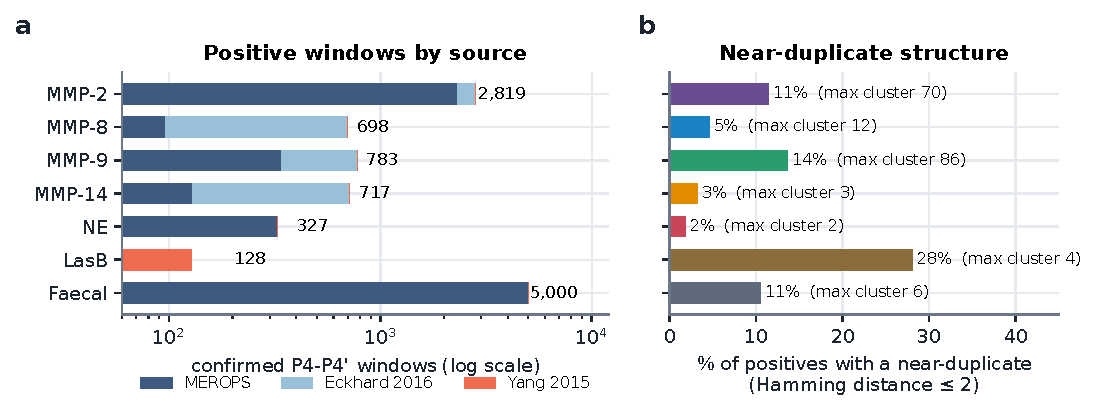
\includegraphics[width=\textwidth]{figures/F02_data_composition.pdf}
\caption{\textbf{(a)} Positive windows per protease by source (log scale). \textbf{(b)} Fraction of positives that have at least one near-duplicate (Hamming distance $\le2$) and the size of the largest cluster.}
\label{fig:data}
\end{figure}

\subsection{How different are the proteases in this data?}
Exact window overlap between protease positive sets is small (Figure~\ref{fig:sim}a; at most a Jaccard index of $0.145$, between MMP-8 and MMP-9), and windows shared with the target are removed from its negatives. But the \emph{position-specific preferences} overlap strongly among the MMPs: the PSSM log-odds vectors of MMP-2, MMP-8 and MMP-14 correlate at $r=0.73$--$0.82$, and MMP-9 correlates at $0.56$--$0.63$ with each (Figure~\ref{fig:sim}b). NE is essentially uncorrelated with the MMPs, and correlates with the faecal group at $0.46$, both being serine proteases. This structure predicts the selectivity results of Section~\ref{sec:res-sel}.

\begin{figure}[!htbp]
\centering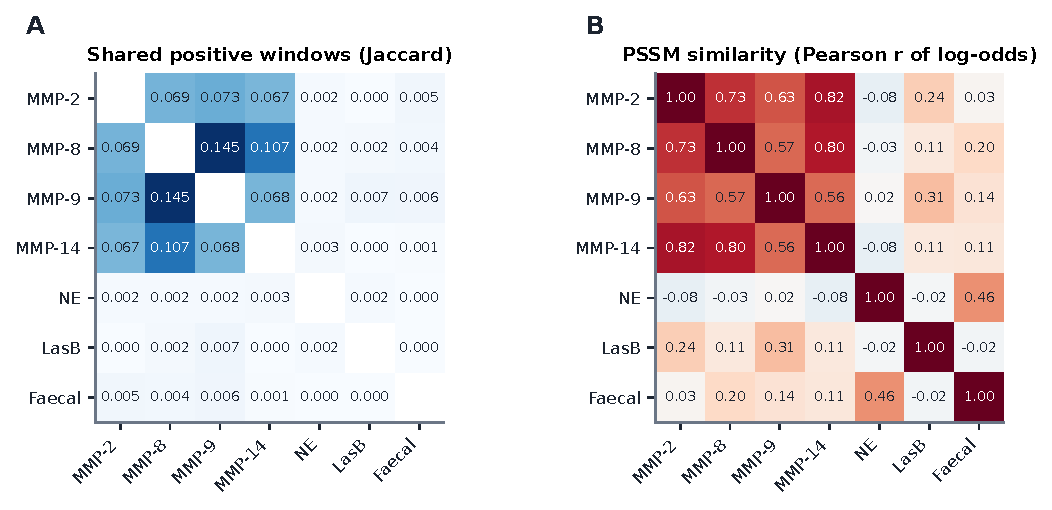
\includegraphics[width=\textwidth]{figures/F04_protease_similarity.pdf}
\caption{\textbf{(a)} Jaccard index of exact positive windows. \textbf{(b)} Pearson correlation of the $8\times20$ PSSM log-odds between protease pairs.}
\label{fig:sim}
\end{figure}

\begin{figure}[!htbp]
\centering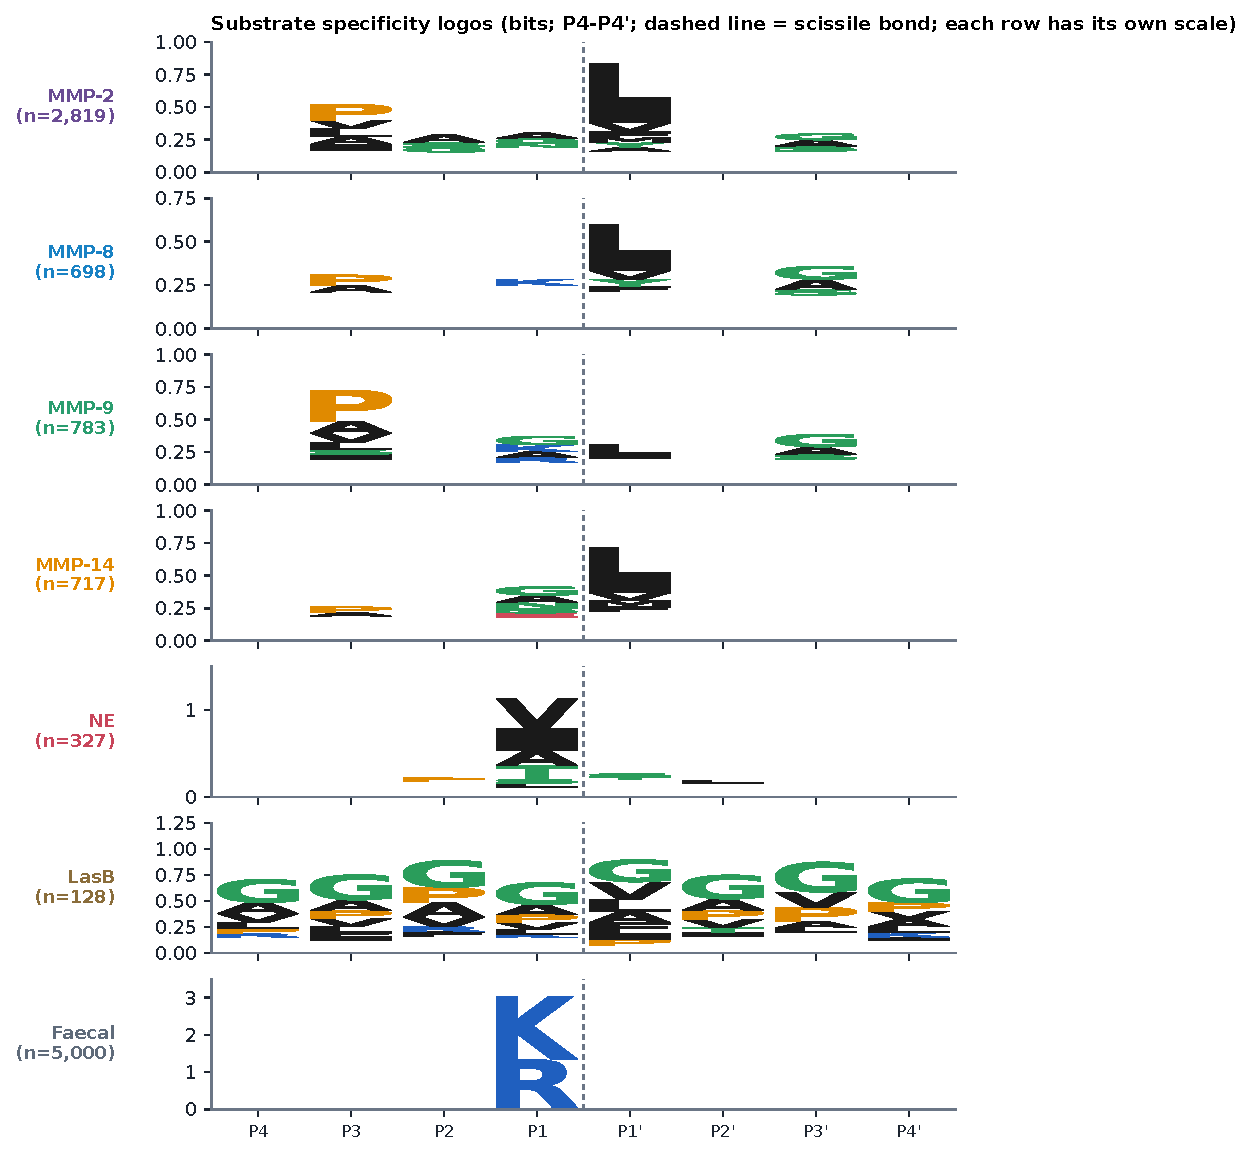
\includegraphics[width=0.86\textwidth]{figures/F03_sequence_logos.pdf}
\caption{Substrate specificity logos computed from each model's PSSM (letter height is probability times information content; each row has its own vertical scale, since the MMPs carry under one bit per position while the faecal group exceeds three at $\pos{1}$). The MMPs share Pro at $\pos{3}$ and a hydrophobic residue at $\prm{1}$; NE prefers small aliphatic residues at $\pos{1}$; the faecal group is dominated by Lys/Arg at $\pos{1}$. The LasB logo is Gly-rich because $97$ of its $128$ positives come from elastin (Section~\ref{sec:limits}).}
\label{fig:logos}
\end{figure}

\section{Models}
\label{sec:models}

\begin{figure}[!htbp]
\centering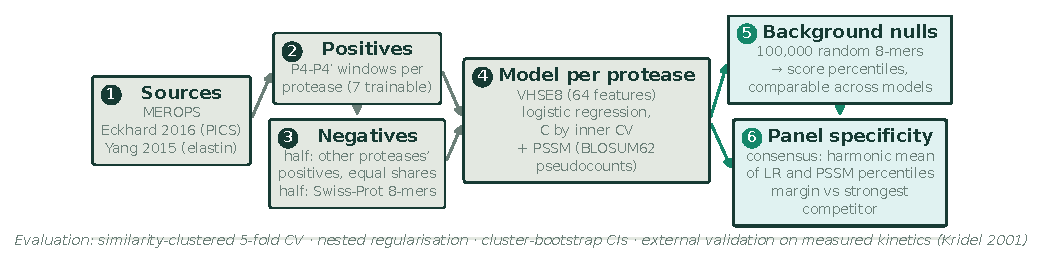
\includegraphics[width=\textwidth]{figures/F01_pipeline.pdf}
\caption{Overview of the pipeline from source data to panel selectivity.}
\label{fig:pipeline}
\end{figure}

\subsection{Physicochemical representation}
Each residue $a$ is mapped to $\varphi(a)\in\R^{8}$, its VHSE descriptor vector: eight principal-component score vectors derived by Mei et al.\ (2005) from independent families of $18$ hydrophobic, $17$ steric and $15$ electronic properties, of which VHSE1--2 are hydrophobic, VHSE3--4 steric and VHSE5--8 electronic. A window $w=(w_1,\dots,w_8)$ becomes
\begin{equation}
\bm{x}(w)=\bigl[\varphi(w_1);\,\varphi(w_2);\,\dots;\,\varphi(w_8)\bigr]\in\R^{64}.
\end{equation}
The descriptor table is archived with its source (\texttt{references/}) and unit-tested against it.

\paragraph{What this encoding can and cannot express.} A linear model on $\bm{x}$ has the additive form $\sum_i c_i^{\top}\varphi(w_i)$, so at each position the effect of the residue is a linear combination of the eight columns of the descriptor matrix $\Phi\in\R^{20\times8}$. Together with a constant, that confines each position's twenty-dimensional effect vector to a subspace of dimension $\operatorname{rank}[\Phi,\bm 1]=9$. A one-hot encoding has no such restriction ($19$ free parameters per position). Projecting each learned PSSM row onto the VHSE subspace shows that it captures $\subspaceMin$--$\subspaceMax\%$ of the variance of the position-specific log-odds, depending on the protease (Table~\ref{tab:controls}). The remaining variance is bias; the reduction from $19$ to $8$ parameters per position is the variance benefit. Section~\ref{sec:res-models} shows both sides of that trade-off empirically.

\subsection{Logistic regression}
\label{sec:lr}
Features are standardised using the training fold's means and standard deviations, $\bm z=(\bm x-\bm\mu)\oslash\bm\sigma$. The classifier minimises the class-weighted, L2-regularised logistic loss
\begin{equation}
\mathcal{L}(\bm\beta,b)=\tfrac12\|\bm\beta\|^2+C\sum_{i=1}^{n}\omega_{y_i}\log\bigl(1+e^{-\tilde y_i(\bm\beta^{\top}\bm z_i+b)}\bigr),\qquad \tilde y_i=2y_i-1,
\label{eq:lr}
\end{equation}
with ``balanced'' class weights $\omega_c=n/(2n_c)$, i.e.\ $\omega_1=2$ and $\omega_0=2/3$ at our $1{:}3$ ratio. The loss is strictly convex in $(\bm\beta,b)$ (its Hessian is $\bm I+C\sum_i\omega_{y_i}p_i(1-p_i)\tilde{\bm z}_i\tilde{\bm z}_i^{\top}\succ0$ with $\tilde{\bm z}=[\bm z;1]$ apart from the unpenalised intercept), so the optimiser (L-BFGS) finds the unique minimum. The regularisation strength $C\in\{10^{-3},\dots,10^{2}\}$ is chosen by an inner cross-validation on the training data only (Section~\ref{sec:cv}).

\begin{derivation}[Meaning of the balanced weights]
Equal total weight on the two classes is equivalent to fitting the posterior under a $50{:}50$ prior. If $\rho=p_{\mathrm{bal}}/(1-p_{\mathrm{bal}})$ is the fitted odds, the odds under the actual $1{:}3$ training mixture are $\rho/3$, so $p_{\mathrm{mix}}=p_{\mathrm{bal}}/(3-2p_{\mathrm{bal}})$. Neither is the probability that a random window is cleaved, which is far smaller. This is why the reliability curves in Figure~\ref{fig:calib} lie away from the diagonal and why we never present the score as a probability.
\end{derivation}

\paragraph{Per-position decomposition.} Because the logit is linear in $\bm z$, it splits exactly into one term per position,
\begin{equation}
\mathrm{logit}(w)=b+\sum_{i=1}^{8}\kappa_i(w),\qquad \kappa_i(w)=\sum_{d=1}^{8}\beta_{id}\,z_{id}(w),
\label{eq:decomp}
\end{equation}
which the interactive tool draws as a bar per position.

\subsection{Position-specific scoring matrix}
For observed residue counts $n_{i}(a)$ among $n$ positives, let $f_i(a)=n_i(a)/n$. Rare residues are smoothed toward a substitution-weighted expectation. Let $W$ be the row-normalised positive part of BLOSUM62, $W_{ab}\propto\max(S_{ab},0)$, and $q_i=f_i W$; mix in the Swiss-Prot background $g$ so that no residue has zero probability:
\begin{equation}
Q_i=(1-\epsilon)\,q_i+\epsilon\,g,\qquad p_i(a)=\frac{n\,f_i(a)+\beta\,Q_i(a)}{n+\beta},\qquad S(w)=\sum_{i=1}^{8}\log_2\frac{p_i(w_i)}{g(w_i)},
\label{eq:pssm}
\end{equation}
with $\beta=5$ pseudo-observations and $\epsilon=0.05$. This is a heuristic pseudocount scheme, not the block-based estimator that BLOSUM62 itself derives from; it is fully specified and unit-tested, and it has no fitted hyperparameter beyond $\beta,\epsilon$. Position $i$ carries $\mathrm{IC}_i=\sum_a p_i(a)\log_2\!\bigl(p_i(a)/g(a)\bigr)$ bits, which sets the letter heights in Figure~\ref{fig:logos}.

\subsection{Background null, percentiles and panel selectivity}
\label{sec:null}
\paragraph{Why raw scores cannot be compared.} Different proteases are trained on different positives and different negatives, so their logits and PSSM scores live on different scales. Even the average LR score on a random window differs by model (Figure~\ref{fig:calib}b), which makes a ratio such as $p_t/\max_{j\ne t}p_j$ depend on the training set of each model rather than on the peptide.

\paragraph{Percentile transform.} For protease $k$ and score $s_k$, let $F_k$ be the distribution function of $s_k(W)$ over random windows $W$ drawn from the background composition. We report $u_k^{\mathrm{LR}}(w)=F_k^{\mathrm{LR}}(s_k^{\mathrm{LR}}(w))$ and $u_k^{\mathrm{PSSM}}(w)=F_k^{\mathrm{PSSM}}(s_k^{\mathrm{PSSM}}(w))$. By the probability integral transform, each is uniform on $[0,1]$ under the null for every protease, so values are directly comparable across models (Appendix~\ref{app:deriv}); each is also invariant to any monotone rescaling of its score. $F_k$ is estimated from $100{,}000$ random windows and stored as a $1{,}001$-point quantile grid, interpolated linearly, so the resolution at the top of the range is $10^{-3}$.

\paragraph{Consensus and margin.} The two percentiles are combined by their harmonic mean,
\begin{equation}
u_k(w)=\frac{2\,u_k^{\mathrm{LR}}(w)\,u_k^{\mathrm{PSSM}}(w)}{u_k^{\mathrm{LR}}(w)+u_k^{\mathrm{PSSM}}(w)},
\label{eq:cons}
\end{equation}
which is high only when both scorers agree. For a target $t$ in a panel $\mathcal{P}$, the specificity margin is
\begin{equation}
M_t(w;\mathcal{P})=u_t(w)-\max_{j\in\mathcal{P}\setminus\{t\}}u_j(w)\ \in[-1,1].
\label{eq:margin}
\end{equation}
A margin near $+1$ means the window is in the extreme tail for the target and near the bulk for every competitor; a margin near $0$ means it is as strongly recognised by some competitor as by the target. The margin depends on the panel by construction.

\subsection{Windows with unknown positions}
Sensor cores are often shorter than eight residues around the bond, so some positions are unknown (marked ``$-$''). Both scorers are additive over positions, which gives a principled treatment. For the logit, an unknown position contributes its training mean, $z_{id}=0$, which equals the expectation of the linear score under any distribution of that feature with the training mean. For the PSSM, an unknown position contributes the background expectation $\sum_a g(a)\log_2(p_i(a)/g(a))$. Percentiles are then taken against a null computed with the \emph{same} positions masked, so that a gapped window is compared with equally uninformed random windows.

\subsection{Portability}
Each trained model is a plain JSON file of arrays (feature means and scales, coefficients, intercept, the $8\times20$ PSSM, and the two quantile grids). The Python package and the browser tool read the same files and are tested for numerical agreement.

\section{Evaluation methodology}
\label{sec:eval}

This section lists what could make the reported performance wrong and the design choice that addresses each threat.

\begin{table}[!htbp]
\centering\small
\begin{tabular}{@{}p{4.1cm}p{5.2cm}p{5.6cm}@{}}\toprule
Threat & Why it matters here & Control \\\midrule
Near-duplicate leakage & Repeats and overlapping peptides let a model memorise neighbours & Folds built over Hamming-distance clusters (Section~\ref{sec:cv}); comparison with random folds \\
Optimistic hyperparameters & Tuning on the evaluation data inflates the estimate & Regularisation chosen in an inner loop that sees only the training fold \\
Optimistic auxiliary models & A PSSM scored on its own training positives is trivially high & PSSM refit in every fold and scored out-of-fold \\
Shortcut features & Composition alone may separate classes & Composition-only and label-shuffled controls \\
Selection among many models & The best of several models is biased upward & All models on identical folds; paired tests; intervals, not point estimates \\
Dependent samples & Ordinary bootstrap treats near-duplicates as independent & Cluster bootstrap for every interval \\
Label noise (PU) & Unlabelled windows may be positives & Analysed formally (Section~\ref{sec:contam}) \\
Scale mismatch across models & Ratios of raw scores are training-set artefacts & Percentile scale; base rates reported \\
External validity & Cross-validation shares the data-generating process & Held-out measured kinetics (Section~\ref{sec:bio-val}) \\\bottomrule
\end{tabular}
\caption{Threats to validity and the control applied to each.}
\end{table}

\subsection{Cluster-aware cross-validation}
\label{sec:cv}
Clusters are the connected components of the Hamming-distance-$\le2$ graph over \emph{all} training windows (positives and negatives). They are computed exactly and efficiently by a pigeonhole argument (Appendix~\ref{app:deriv}): two windows differing at at most two of eight positions must agree exactly on at least one of three blocks of sizes $3,3,2$, so only windows sharing a block need be compared. Folds are drawn with stratified group $5$-fold cross-validation over the clusters, so that no cluster straddles a train/test boundary and each fold keeps the class ratio. Every reported AUROC, PR-AUC, MCC and Brier score is computed on out-of-fold predictions pooled across the five folds.

\subsection{Nested regularisation and per-fold auxiliary models}
Within each outer training set, the logistic-regression $C$ is chosen from $\{10^{-3},\dots,10^{2}\}$ by an inner $3$-fold cluster-aware cross-validation (mean AUROC), and only then is the model refit on the whole outer training set and applied to the outer test fold. The PSSM is rebuilt from the positives of each training fold. The background null used for percentiles is likewise rebuilt per fold from that fold's models ($5{,}000$ random windows), so the cross-validated consensus score uses no information from its test fold.

\subsection{Metrics}
\emph{AUROC} is the probability that a random positive outranks a random negative (equal to the Mann--Whitney statistic; Appendix~\ref{app:deriv}); it is threshold-free and insensitive to the arbitrary $1{:}3$ ratio. \emph{PR-AUC} is reported against a positive prior of $0.25$. \emph{MCC} uses the logistic-regression score at the fixed threshold $0.5$ and is therefore only indicative under balanced class weighting. The \emph{Brier score} and the \emph{expected calibration error} (ECE) describe agreement between score and outcome under the training prior and are reported to show that scores are not probabilities.

\subsection{Uncertainty and comparisons}
Intervals are $95\%$ cluster-bootstrap intervals: whole clusters are resampled with replacement ($500$ replicates), which respects the dependence that an ordinary bootstrap ignores. When two models are compared, the same resampled clusters are used for both and the interval is for the difference in AUROC (paired cluster bootstrap, $400$ replicates); a difference is called significant when its $95\%$ interval excludes zero. We make no multiplicity correction across the $35$ paired comparisons ($5$ alternatives $\times$ $7$ proteases; $28$ are shown in Table~\ref{tab:paired}); readers should treat isolated borderline results accordingly.

\subsection{External validation protocol}
Section~\ref{sec:bio-val} compares model scores with kinetics measured on peptides that were \emph{not} in the training data. Before scoring, every training window (positive or cross-negative, any protease) that coincides with a validation peptide on at least seven of its positions is removed and the model is retrained, so the validation set cannot leak into training; four windows were removed. Peptides shorter than eight positions around the bond are scored as gapped windows (Section~\ref{sec:null}).

\section{Results}
\label{sec:results}

\subsection{Detection performance}
\label{sec:res-main}
Table~\ref{tab:main} gives cluster-aware, out-of-fold AUROC for the logistic regression, the PSSM, and their consensus (Eq.~\ref{eq:cons}). Discrimination is well above chance for every protease, ranging from \aucConsMMPnine{} for MMP-9 to \aucConsFaecal{} for the faecal group. The serine-protease models (NE, faecal) and LasB are best, the MMPs least so. The consensus is at or near the best single scorer for all proteases; for MMP-2 and MMP-8 the PSSM alone is slightly higher, with overlapping intervals. Secondary metrics are in Table~\ref{tab:secondary}; Figure~\ref{fig:roc} shows ROC and precision-recall curves.

\begin{table}[!htbp]
\centering\small{\footnotesize\begin{tabular}{@{}lrrccc@{}}\toprule
Protease & Positives & Positive clusters & LR AUROC & PSSM AUROC & Consensus AUROC \\\midrule
MMP-2 & 2,819 & 2,608 & 0.854 \,[0.844, 0.863] & \textbf{0.874 \,[0.863, 0.883]} & 0.869 \,[0.859, 0.878] \\
MMP-8 & 698 & 677 & 0.755 \,[0.733, 0.774] & \textbf{0.784 \,[0.762, 0.800]} & 0.783 \,[0.763, 0.800] \\
MMP-9 & 783 & 687 & 0.760 \,[0.723, 0.791] & 0.761 \,[0.723, 0.798] & \textbf{0.772 \,[0.737, 0.803]} \\
MMP-14 & 717 & 705 & 0.772 \,[0.753, 0.790] & 0.785 \,[0.766, 0.806] & \textbf{0.791 \,[0.771, 0.810]} \\
Neutrophil elastase & 327 & 324 & 0.895 \,[0.875, 0.913] & 0.885 \,[0.861, 0.906] & \textbf{0.901 \,[0.880, 0.919]} \\
LasB & 128 & 106 & 0.877 \,[0.835, 0.917] & 0.881 \,[0.837, 0.916] & \textbf{0.887 \,[0.844, 0.923]} \\
Faecal serine proteases & 5,000 & 4,715 & 0.951 \,[0.948, 0.954] & 0.953 \,[0.950, 0.956] & \textbf{0.953 \,[0.950, 0.956]} \\
\bottomrule\end{tabular}}

\caption{Cluster-aware $5$-fold cross-validated AUROC with $95\%$ cluster-bootstrap intervals (bold: highest of the three scorers). ``Positive clusters'' is the number of distinct near-duplicate clusters among the positives.}
\label{tab:main}
\end{table}

\begin{table}[!htbp]
\centering\small\begin{tabular}{@{}lccccl@{}}\toprule
Protease & PR-AUC & MCC & Brier & ECE & $C$ chosen per outer fold \\\midrule
MMP-2 & 0.649 & 0.521 & 0.156 & 0.153 & 0.1, 0.1, 0.1, 0.1, 0.1 \\
MMP-8 & 0.474 & 0.346 & 0.202 & 0.199 & 0.01, 0.01, 0.01, 0.01, 0.01 \\
MMP-9 & 0.535 & 0.335 & 0.196 & 0.196 & 0.01, 0.01, 0.01, 0.01, 0.01 \\
MMP-14 & 0.516 & 0.370 & 0.195 & 0.191 & 0.1, 0.01, 0.01, 0.1, 0.01 \\
Neutrophil elastase & 0.751 & 0.600 & 0.127 & 0.114 & 0.1, 0.1, 0.1, 0.1, 0.1 \\
LasB & 0.783 & 0.602 & 0.125 & 0.122 & 0.01, 0.1, 0.1, 0.1, 0.01 \\
Faecal serine proteases & 0.800 & 0.806 & 0.071 & 0.055 & 1.0, 0.1, 1.0, 0.1, 0.1 \\
\bottomrule\end{tabular}

\caption{Secondary metrics for the logistic regression. PR-AUC is measured against a prior of $0.25$; MCC at threshold $0.5$; ECE under the training prior. Selected $C$ is listed per outer fold.}
\label{tab:secondary}
\end{table}

\begin{figure}[!htbp]
\centering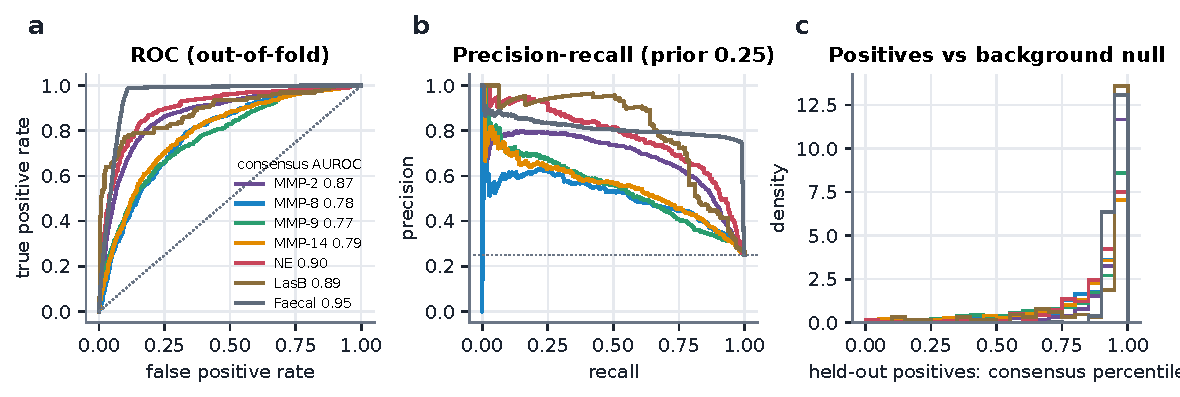
\includegraphics[width=\textwidth]{figures/F09_roc_pr.pdf}
\caption{Out-of-fold performance of the consensus score. \textbf{(a)} ROC curves. \textbf{(b)} Precision-recall curves. \textbf{(c)} Distribution of the consensus percentile of held-out positives; positives concentrate near the top of the background distribution for every protease.}
\label{fig:roc}
\end{figure}

\subsection{Which model, and which representation?}
\label{sec:res-models}
Figure~\ref{fig:models} and Table~\ref{tab:models} compare seven models on identical folds: a constant prior, a composition-only logistic regression, one-hot and VHSE logistic regressions, the PSSM, and gradient-boosted trees on both encodings. Three conclusions follow.

\begin{enumerate}
\item \textbf{Position matters; composition mostly does not.} For six of seven proteases, composition alone gives $0.60$--$0.74$ AUROC and the VHSE model beats it significantly (Table~\ref{tab:paired}); label-shuffled controls sit at chance (Table~\ref{tab:controls}). \textbf{LasB is the exception:} composition alone reaches $0.886$, statistically indistinguishable from the full model ($-0.008$, interval including zero). The LasB model is largely detecting elastin-like composition, as expected from a positive set that is $76\%$ elastin (Section~\ref{sec:limits}).
\item \textbf{There is no evidence of strong position--position interaction.} Gradient-boosted trees, which can represent interactions, reach within $0.013$ AUROC of the better of the one-hot regression and the PSSM on every protease and exceed it only on NE, by $0.007$. An additive model is adequate at these data sizes, and it is also the interpretable one.
\item \textbf{The representation trade-off is real.} On data-rich proteases (MMP-2, MMP-8) the one-hot logistic regression and the PSSM are significantly better than the VHSE model by $0.017$ to $0.034$ AUROC, consistent with the bias measured in Table~\ref{tab:controls}. On NE and LasB the VHSE model is significantly better than the one-hot model ($+0.021$ and $+0.033$). The learning curves (Figure~\ref{fig:lc}) show the same crossover: VHSE is ahead at small training sizes and is overtaken as data grow.
\end{enumerate}
The PSSM has no fitted hyperparameter and is at or within its interval of the best model everywhere, which is why the shipped score combines it with the logistic regression rather than choosing one.

\begin{figure}[!htbp]
\centering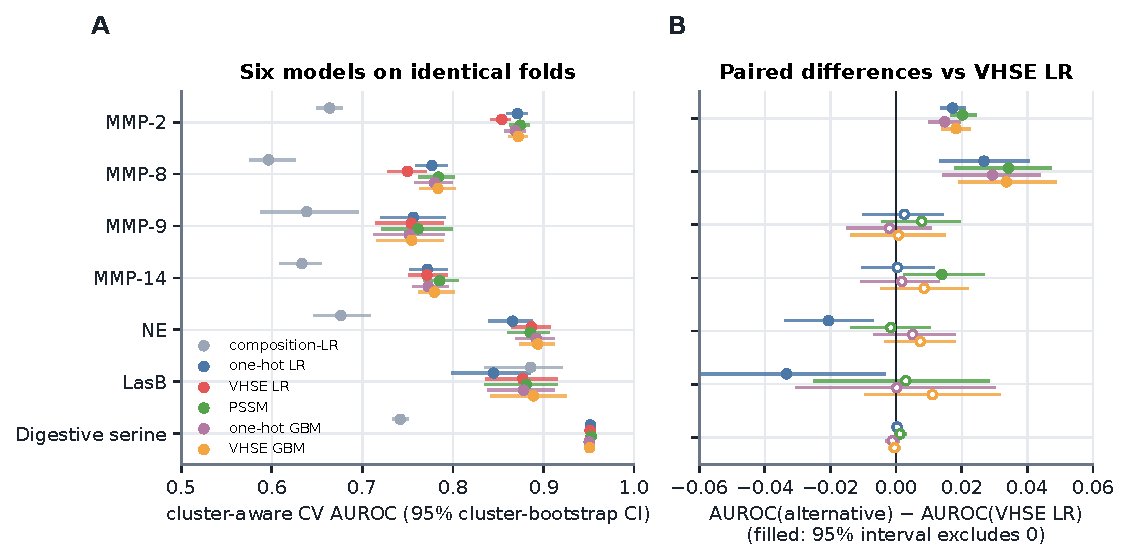
\includegraphics[width=\textwidth]{figures/F05_model_comparison.pdf}
\caption{\textbf{(a)} Cluster-aware AUROC of six models on identical folds with $95\%$ cluster-bootstrap intervals. \textbf{(b)} Paired difference (alternative minus VHSE LR); filled markers have intervals excluding zero. The composition-only model is $0.12$--$0.21$ AUROC below for every protease except LasB and is omitted from panel (b) for scale.}
\label{fig:models}
\end{figure}

\begin{table}[!htbp]
\centering\small\begin{tabular}{@{}lccccccc@{}}\toprule
Protease & Prior & Composition & One-hot LR & VHSE LR & PSSM & One-hot GBM & VHSE GBM \\\midrule
MMP-2 & 0.500 & 0.664 & 0.871 & 0.854 & \textbf{0.874} & 0.869 & 0.872 \\
MMP-8 & 0.500 & 0.596 & 0.777 & 0.750 & \textbf{0.784} & 0.780 & 0.783 \\
MMP-9 & 0.500 & 0.639 & 0.756 & 0.754 & \textbf{0.761} & 0.752 & 0.755 \\
MMP-14 & 0.500 & 0.633 & 0.772 & 0.771 & \textbf{0.785} & 0.773 & 0.779 \\
Neutrophil elastase & 0.500 & 0.676 & 0.866 & 0.887 & 0.885 & 0.892 & \textbf{0.894} \\
LasB & 0.500 & 0.886 & 0.845 & 0.877 & 0.881 & 0.878 & \textbf{0.889} \\
Faecal serine proteases & 0.500 & 0.742 & 0.952 & 0.951 & \textbf{0.953} & 0.950 & 0.951 \\
\bottomrule\end{tabular}

\caption{Cross-validated AUROC by model and protease (bold: best). The prior is constant and gives $0.5$.}
\label{tab:models}
\end{table}

\begin{table}[!htbp]
\centering\small\begin{tabular}{@{}lcccc@{}}\toprule
Protease & One-hot LR & PSSM & One-hot GBM & VHSE GBM \\\midrule
MMP-2 & +0.017$^{*}$ & +0.020$^{*}$ & +0.015$^{*}$ & +0.018$^{*}$ \\
MMP-8 & +0.027$^{*}$ & +0.034$^{*}$ & +0.029$^{*}$ & +0.034$^{*}$ \\
MMP-9 & +0.003 & +0.008 & -0.002 & +0.001 \\
MMP-14 & +0.000 & +0.014$^{*}$ & +0.002 & +0.009 \\
Neutrophil elastase & -0.021$^{*}$ & -0.002 & +0.005 & +0.007 \\
LasB & -0.033$^{*}$ & +0.003 & +0.000 & +0.011 \\
Faecal serine proteases & +0.000 & +0.001 & -0.001 & -0.000 \\
\bottomrule\end{tabular}

\caption{AUROC of each alternative minus the VHSE logistic regression, with a paired cluster bootstrap (the composition-only model, which is far below, is omitted). $^{*}$: $95\%$ interval excludes zero. No multiplicity correction is applied.}
\label{tab:paired}
\end{table}

\begin{figure}[!htbp]
\centering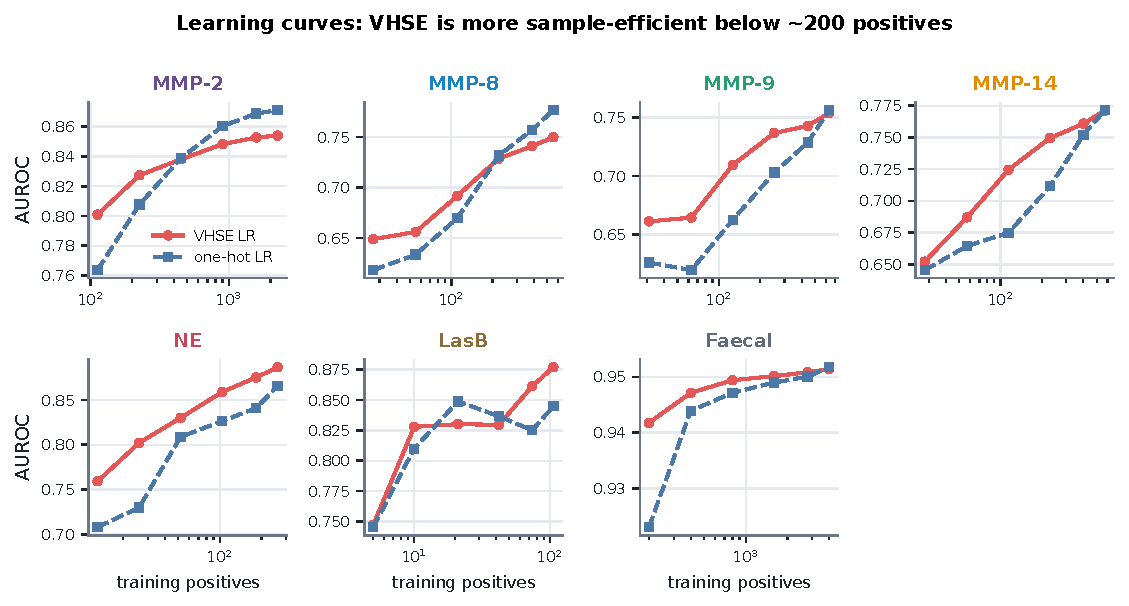
\includegraphics[width=\textwidth]{figures/F06_learning_curves.pdf}
\caption{Learning curves: AUROC as a function of the number of training positives for the VHSE and one-hot logistic regressions. The physicochemical encoding is more sample-efficient at small sizes.}
\label{fig:lc}
\end{figure}

\subsection{Training against other proteases}
\label{sec:res-neg}
The training negatives determine what the model learns to reject. We compare three designs on a \emph{common} held-out test set, trained inside identical folds: (i) composition-shuffled positives plus background (the design used in earlier work), (ii) background only, and (iii) our panel design. Each is scored on held-out target positives against (a) background windows and (b) held-out positives of the other proteases (Table~\ref{tab:neg}, Figure~\ref{fig:neg}). The panel design costs $0.01$--$0.02$ AUROC against background but gains against competitors on every protease, most where it matters: for LasB from $0.80$ (background only) and $0.68$ (shuffled) to $0.86$, for MMP-14 from $0.65$ to $0.73$, and for MMP-2 from $0.76$ to $0.79$.

\begin{table}[!htbp]
\centering\small\begin{tabular}{@{}lcccccc@{}}\toprule
 & \multicolumn{2}{c}{Shuffled + background} & \multicolumn{2}{c}{Background only} & \multicolumn{2}{c}{Panel (ours)} \\
\cmidrule(lr){2-3}\cmidrule(lr){4-5}\cmidrule(lr){6-7}
Protease & vs bkg & vs comp. & vs bkg & vs comp. & vs bkg & vs comp. \\\midrule
MMP-2 & 0.881 & 0.756 & 0.885 & 0.762 & 0.882 & 0.787 \\
MMP-8 & 0.834 & 0.654 & 0.828 & 0.651 & 0.810 & 0.683 \\
MMP-9 & 0.819 & 0.660 & 0.832 & 0.667 & 0.816 & 0.683 \\
MMP-14 & 0.831 & 0.660 & 0.833 & 0.649 & 0.811 & 0.727 \\
Neutrophil elastase & 0.850 & 0.910 & 0.852 & 0.900 & 0.848 & 0.926 \\
LasB & 0.801 & 0.676 & 0.889 & 0.798 & 0.891 & 0.863 \\
Faecal serine proteases & 0.954 & 0.939 & 0.954 & 0.938 & 0.953 & 0.944 \\
\bottomrule\end{tabular}

\caption{Held-out AUROC by negative-set design against random background (bkg) and against other proteases' substrates (comp.).}
\label{tab:neg}
\end{table}

\begin{figure}[!htbp]
\centering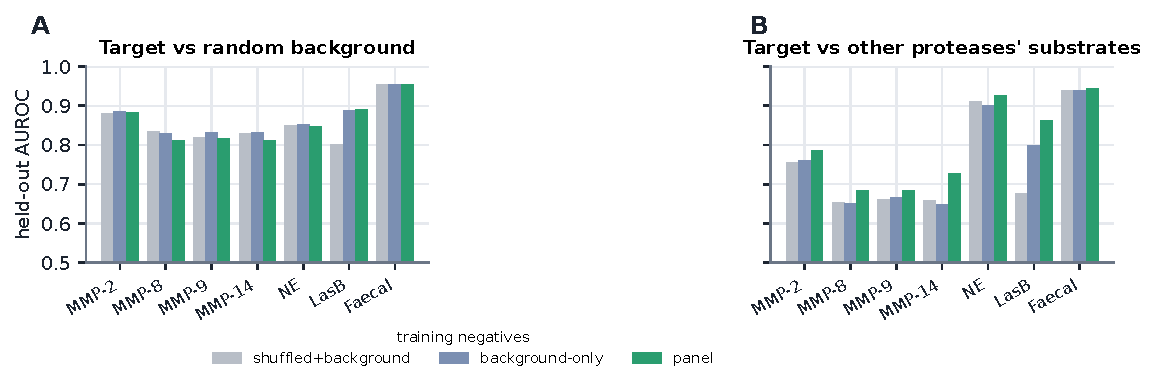
\includegraphics[width=\textwidth]{figures/F07_negative_design.pdf}
\caption{Effect of the training negatives on detection (a) and cross-protease discrimination (b).}
\label{fig:neg}
\end{figure}

\subsection{Regularisation, leakage and controls}
Choosing $C$ by inner cross-validation raises or matches the $C=1$ default (Table~\ref{tab:controls}, Figure~\ref{fig:tune}), selecting $C=0.01$--$0.1$ for every protease except the faecal group (strong regularisation for a $64$-feature model on hundreds of examples). Random and cluster-aware folds differ by at most \maxLeakGap{} AUROC, so near-duplicate leakage is not a material source of optimism in these data, even though the folds guard against it. Label-shuffled models score \shuffleMin--\shuffleMax{}.

\begin{table}[!htbp]
\centering\small\begin{tabular}{@{}lcccccc@{}}\toprule
 & \multicolumn{2}{c}{Regularisation} & \multicolumn{2}{c}{Fold construction} & Label & VHSE span \\
\cmidrule(lr){2-3}\cmidrule(lr){4-5}
Protease & $C=1$ & nested & random & clustered & shuffle & coverage \\\midrule
MMP-2 & 0.854 & 0.854 & 0.855 & 0.854 & 0.505 & 79\% \\
MMP-8 & 0.750 & 0.755 & 0.752 & 0.752 & 0.493 & 64\% \\
MMP-9 & 0.754 & 0.760 & 0.755 & 0.756 & 0.493 & 64\% \\
MMP-14 & 0.771 & 0.772 & 0.771 & 0.773 & 0.509 & 79\% \\
Neutrophil elastase & 0.887 & 0.895 & 0.897 & 0.895 & 0.495 & 65\% \\
LasB & 0.877 & 0.877 & 0.886 & 0.879 & 0.526 & 65\% \\
Faecal serine proteases & 0.951 & 0.951 & 0.951 & 0.951 & 0.494 & 77\% \\
\bottomrule\end{tabular}

\caption{Controls. Regularisation: AUROC with $C=1$ versus $C$ chosen in the inner loop. Fold construction: random versus cluster-aware folds (fixed $C=0.1$). Label shuffle: mean over five permutations. VHSE span: variance-weighted share of the learned PSSM log-odds that lies within the VHSE subspace.}
\label{tab:controls}
\end{table}

\begin{figure}[!htbp]
\centering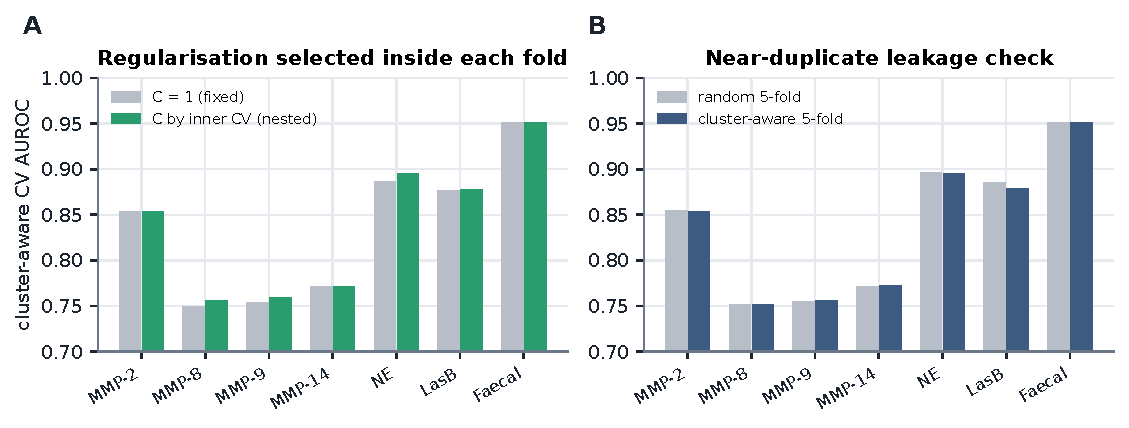
\includegraphics[width=\textwidth]{figures/F08_tuning_and_leakage.pdf}
\caption{\textbf{(a)} Nested regularisation selection versus fixed $C=1$. \textbf{(b)} Random versus cluster-aware folds.}
\label{fig:tune}
\end{figure}

\subsection{Calibration and scale}
\label{sec:res-calib}
Reliability curves of the logistic-regression score lie below the diagonal (Figure~\ref{fig:calib}a): with balanced class weights the score is a posterior under a $50{:}50$ prior, whereas the training mixture has a positive prior of $0.25$ and real sequences far lower. Expected calibration error is $0.06$--$0.20$ (Table~\ref{tab:secondary}). Base rates also differ by model: the mean score on random windows ranges from $0.11$ (faecal) to $0.35$ (MMP-14) (Figure~\ref{fig:calib}b), which is precisely what makes raw probability ratios unsuitable as selectivity measures and motivates the percentile scale.

\begin{figure}[!htbp]
\centering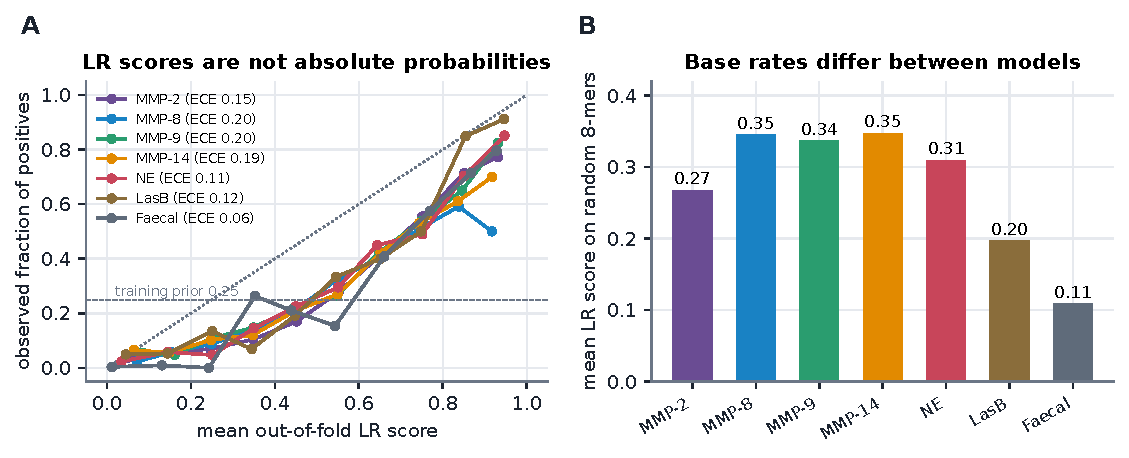
\includegraphics[width=\textwidth]{figures/F10_calibration.pdf}
\caption{\textbf{(a)} Reliability curves of the out-of-fold logistic-regression score. \textbf{(b)} Mean logistic-regression score on random background windows for each final model.}
\label{fig:calib}
\end{figure}

\subsection{Selectivity between proteases}
\label{sec:res-sel}
Table~\ref{tab:selmat} and Figure~\ref{fig:selmat} report, for each target model, the held-out AUROC for separating the target's substrates from a competitor's substrates (the competitor's windows were in training as negatives, but each is scored out-of-fold). The pattern follows the biology of Section~\ref{sec:bio}. The NE and faecal models separate their own substrates from every competitor's at $0.90$--$0.98$. The MMP models separate theirs from NE's at $0.89$--$0.93$, but from LasB's and the faecal group's at only $0.63$--$0.89$. And \emph{within} the MMP family discrimination is modest ($0.53$--$0.72$), lowest for MMP-14 versus MMP-2 ($0.53$) and MMP-8 versus MMP-2 ($0.57$).

\begin{table}[!htbp]
\centering\small\begin{tabular}{@{}lccccccc@{}}\toprule
Target model & MMP-2 & MMP-8 & MMP-9 & MMP-14 & NE & LasB & Faecal \\\midrule
MMP-2 & -- & 0.72 & 0.68 & 0.69 & 0.93 & 0.79 & 0.89 \\
MMP-8 & 0.57 & -- & 0.58 & 0.64 & 0.91 & 0.82 & 0.63 \\
MMP-9 & 0.59 & 0.65 & -- & 0.70 & 0.90 & 0.63 & 0.63 \\
MMP-14 & 0.53 & 0.62 & 0.70 & -- & 0.89 & 0.80 & 0.84 \\
Neutrophil elastase & 0.93 & 0.93 & 0.93 & 0.94 & -- & 0.92 & 0.96 \\
LasB & 0.84 & 0.90 & 0.81 & 0.84 & 0.87 & -- & 0.91 \\
Faecal & 0.96 & 0.90 & 0.91 & 0.96 & 0.98 & 0.97 & -- \\
\bottomrule\end{tabular}

\caption{Held-out AUROC for separating the row protease's substrates from the column protease's substrates.}
\label{tab:selmat}
\end{table}

\begin{figure}[!htbp]
\centering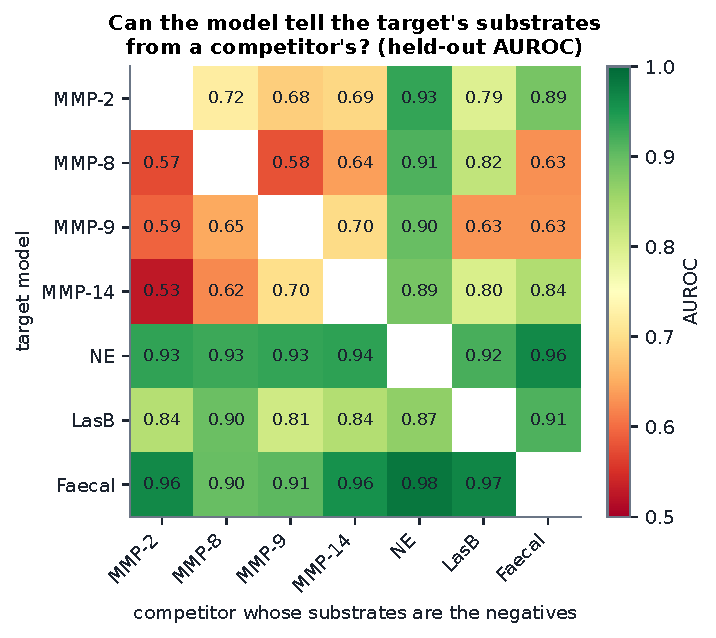
\includegraphics[width=0.62\textwidth]{figures/F11_selectivity_matrix.pdf}
\caption{Cross-protease discrimination matrix (same data as Table~\ref{tab:selmat}).}
\label{fig:selmat}
\end{figure}

\subsubsection{How to read a low competitor AUROC}
\label{sec:contam}
A low value does not by itself indicate a poor model. By Eq.~\eqref{eq:contam-main}, if a fraction $\pi$ of a competitor's substrates are also cleaved by the target, the measured AUROC is at most $(1-\pi)\cdot1+\tfrac12\pi=1-\pi/2$ even for a perfect model. Exact-window overlap between protease positive sets is small (Section~\ref{sec:data}), but the MMPs share their dominant preferences (Section~\ref{sec:bio}), so many unlabelled or ``competitor'' windows are plausibly cleaved by the target as well; the ceiling for MMP-versus-MMP AUROC is therefore below $1$ by an amount we cannot measure from sequence data alone. In other words, part of the within-MMP figure reflects genuine biological promiscuity in the labels. Either way, the practical conclusion is the same: from a P4--P4$'$ window alone, the MMPs cannot be reliably told apart, and a sensor design should not depend on it.

\begin{figure}[!htbp]
\centering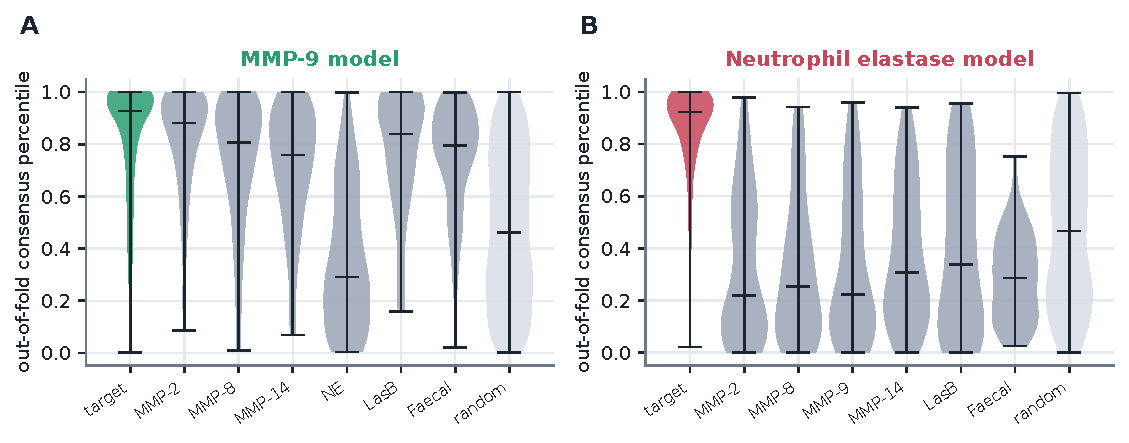
\includegraphics[width=\textwidth]{figures/F16_score_distributions.pdf}
\caption{Out-of-fold consensus percentiles of held-out positives (``target'') and of each competitor's substrates and random windows, for the MMP-9 model (a) and the NE model (b). The MMP-9 model places MMP-2 and MMP-8 substrates almost as high as its own; the NE model separates them sharply.}
\label{fig:dist}
\end{figure}

\subsection{What the models learned}
\label{sec:interp}
Coefficient stability by cluster bootstrap (Figure~\ref{fig:coef}) shows which learned effects are reliable: between $17$ (MMP-14) and $35$ (MMP-2) of the $64$ standardised coefficients per model have intervals excluding zero, so most individual coefficients are not reliably nonzero and the position-level pattern is more trustworthy than any single descriptor weight. Figure~\ref{fig:pos} shows that the total contribution is concentrated at $\pos{3}$ and $\prm{1}$ for the MMPs, at $\pos{1}$ for NE and the faecal group, and is spread across positions for LasB; the electronic family, which accounts for four of the eight descriptors, carries the largest share for every protease.

\begin{figure}[!htbp]
\centering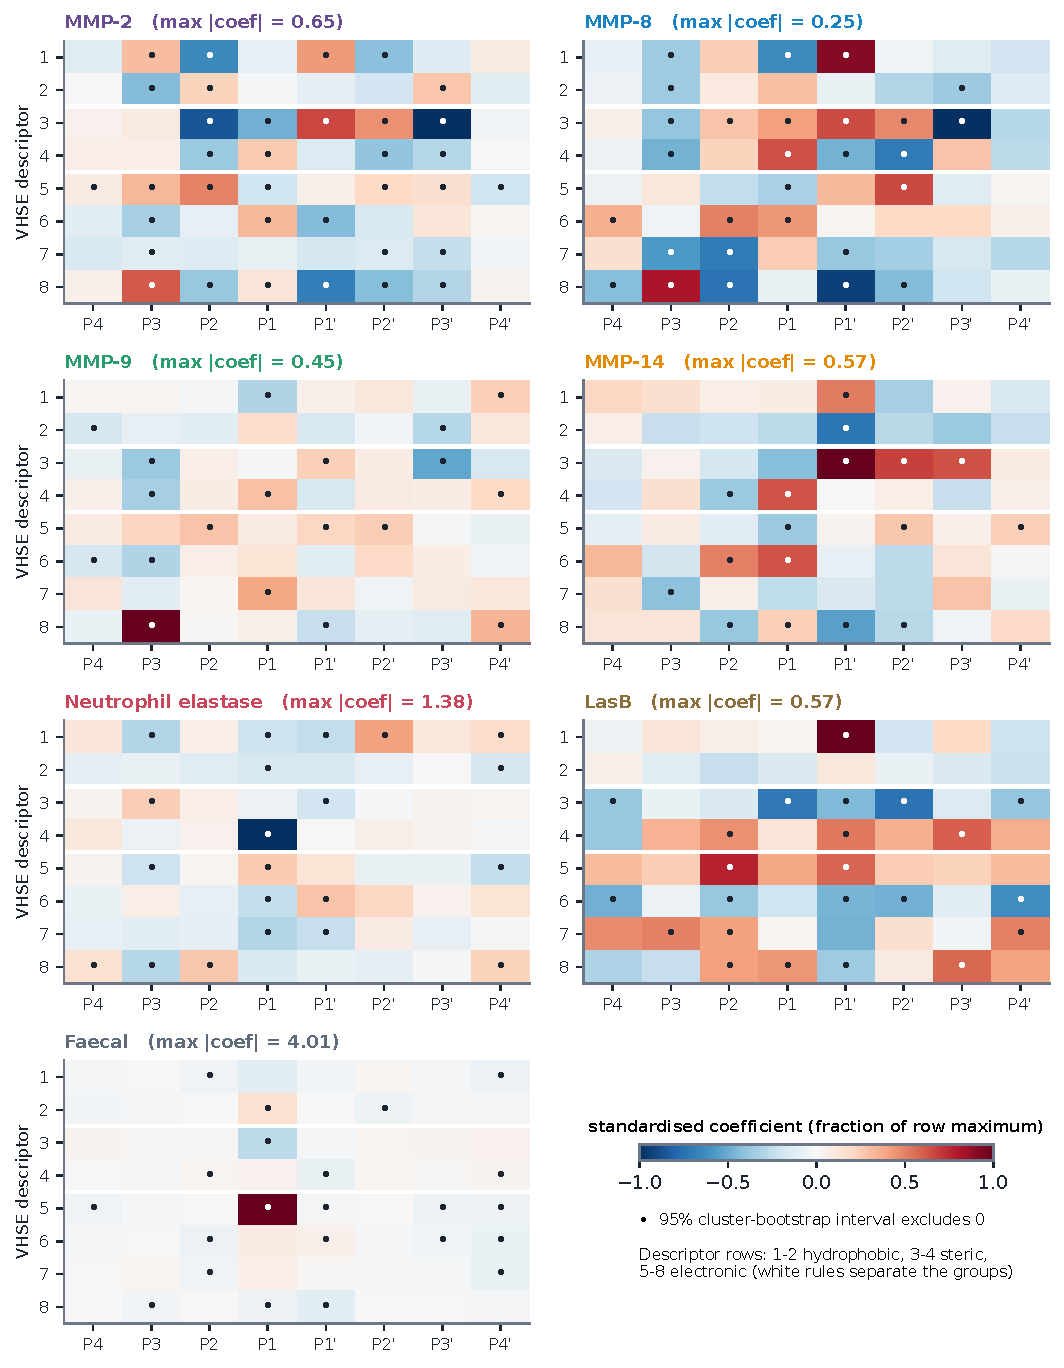
\includegraphics[width=0.97\textwidth]{figures/F12_coefficients.pdf}
\caption{Standardised logistic-regression coefficients by position and VHSE descriptor. Dots mark coefficients whose $95\%$ cluster-bootstrap interval excludes zero. Colours are scaled to each protease's largest coefficient.}
\label{fig:coef}
\end{figure}

\begin{figure}[!htbp]
\centering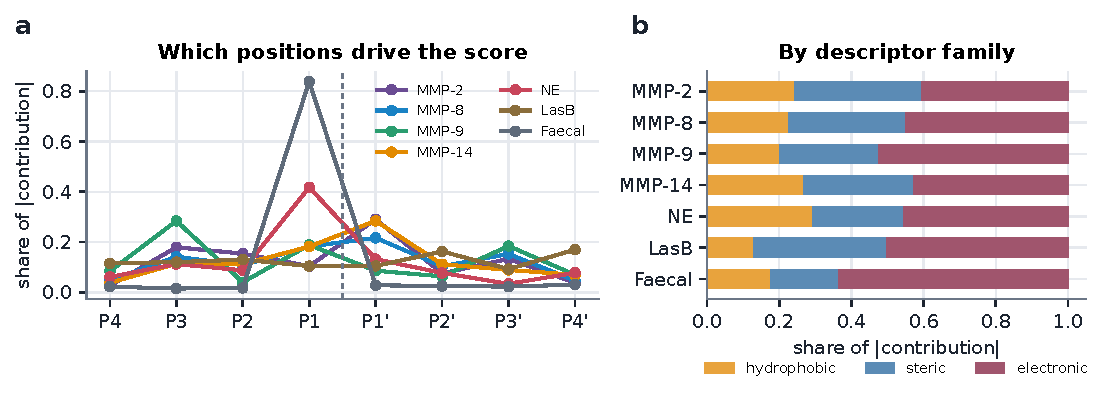
\includegraphics[width=\textwidth]{figures/F13_position_importance.pdf}
\caption{\textbf{(a)} Share of mean absolute logit contribution by position, computed on training positives. \textbf{(b)} Share by descriptor family.}
\label{fig:pos}
\end{figure}

\section{Does the model agree with what is known about these enzymes?}
\label{sec:bio-val}

Cross-validation shows that the model generalises within its data-generating process. This section asks three questions that do not share that process: does it recover published specificity it was not shown, does the structural biology of the enzymes agree with what it learned, and does it rank measured kinetics.

\subsection{Recovery of the MMP-9 consensus}
The phage-display consensus of Kridel et al.\ (2001), Pro-Arg-Ser/Thr$\downarrow$Hy-Ser/Thr, was derived from a different experiment and is not in our training data (MEROPS and PICS). Figure~\ref{fig:kcons} overlays it on the learned MMP-9 PSSM. Pro at $\pos{3}$ is the top-ranked residue of twenty ($+\pssmLOPThreePro$ bits), Leu and Ile are the first and second choices at $\prm{1}$ ($\pssmLOPOnePLeu$ and $\pssmLOPOnePIle$), and Arg at $\pos{2}$ is ranked \pssmRankPTwoArg{}\,/\,20 ($\pssmLOPTwoArg$). These are the two features Kridel et al.\ tie to specific enzyme pockets (an S3 subsite that accommodates the bend introduced by Pro, and the deep hydrophobic S1$'$ pocket).

The model does \emph{not} reproduce Ser/Thr at $\pos{1}$ (Thr ranks \pssmRankPOneThr{}\,/\,20, $\pssmLOPOneThr$; Ser is 9th) or at $\prm{2}$ (Ser ranks \pssmRankPTwoPSer{}\,/\,20, Thr \pssmRankPTwoPThr{}\,/\,20). We do not read this as a failure. Kridel et al.\ note that about two thirds of the $\prm{2}$ Thr residues in their selected clones are encoded by the phage vector rather than selected, so the phage consensus over-represents Thr there. At $\pos{1}$ our top residues are Gly, Lys and Arg (\pssmLOPOneGly{}, \pssmLOPOneLys{}, \pssmLOPOneArg{} bits); Gly at $\pos{1}$ is what the natural collagen and other protein substrates in Kridel et al.'s Table~III show (Pro-X-Gly$\downarrow$Hy), and Arg at $\pos{1}$ is favoured in their group~III substrates. The learned specificity is that of natural and proteome-derived sites, which differs from a phage-optimised consensus in exactly the places one would expect.

\begin{figure}[!htbp]
\centering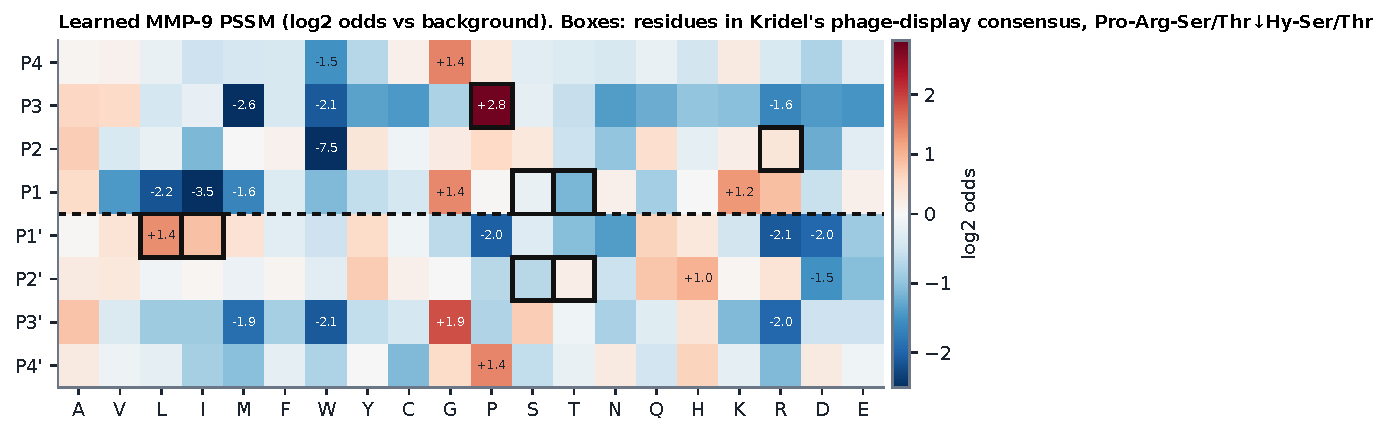
\includegraphics[width=\textwidth]{figures/F14_mmp9_consensus.pdf}
\caption{Learned MMP-9 PSSM (log$_2$ odds against background; only cells with $|{\cdot}|>1$ bit are annotated). Boxes mark the residues of the Kridel et al.\ phage-display consensus. Pro at $\pos{3}$ and Leu/Ile at $\prm{1}$ are recovered; Ser/Thr at $\pos{1}$ and $\prm{2}$ are not (see text).}
\label{fig:kcons}
\end{figure}

\subsection{Learned specificity in the context of the enzyme structures}
\label{sec:structures}
We prepared one experimental structure per protease (Table~\ref{tab:struct}; Figure~\ref{fig:struct}) and derived active-site facts from the coordinates rather than asserting them. In MMP-9, MMP-2 and MMP-8 the sequence around the catalytic zinc reads H-E-F-G-H-A-L-G-L-D/E-H, i.e.\ the HEXXHXXGXXH motif of Nagase and Woessner (1999); the zinc is coordinated by the two histidines of HEXXH and the third histidine of the motif (His401, His405, His411 in MMP-9), and the hydroxamate oxygen of the bound MMP-9 inhibitor lies $2.07$~\AA\ from it. In LasB the zinc ligands are His140, His144 and Glu164; in neutrophil elastase the catalytic triad is His57, Asp102 and Ser195. Residues lining the ligand-occupied pocket of MMP-9 include Asp185-Gly186-Leu187, the Asp-Gly-Leu segment that Kridel et al.\ assign to the S2$'$ subsite (their numbering differs), and Met422. In NE they include Val190, Ala213 and Val216, small aliphatic side chains, and the NE model's top residues at $\pos{1}$ are Val, Ile and Thr (Appendix Table~\ref{tab:topres}).

\begin{table}[!htbp]
\centering\small\begin{tabular}{@{}llcclc@{}}\toprule
Protease & PDB & Resolution (\AA) & Residues & Catalytic site residues & Pocket residues \\\midrule
MMP-2 & 1QIB & 2.8 & 160 & HIS201, HIS205, HIS211 & 23 \\
MMP-8 & 1JAN & 2.5 & 164 & HIS197, HIS201, HIS207 & 21 \\
MMP-9 & 1GKC & 2.3 & 159 & HIS401, HIS405, HIS411 & 20 \\
Neutrophil elastase & 1HNE & 1.84 & 210 & ASP102, HIS57, SER195 & 22 \\
LasB & 1EZM & 1.5 & 298 & GLU164, HIS140, HIS144 & 27 \\
\bottomrule\end{tabular}

\caption{Structures used. The catalytic-site residues are those coordinating the catalytic zinc (MMPs, LasB) or forming the catalytic triad (NE), identified from the coordinates. ``Pocket residues'' are within $6$~\AA\ of the bound ligand, or within $9$~\AA\ of the catalytic zinc when no ligand is present.}
\label{tab:struct}
\end{table}

\begin{figure}[!htbp]
\centering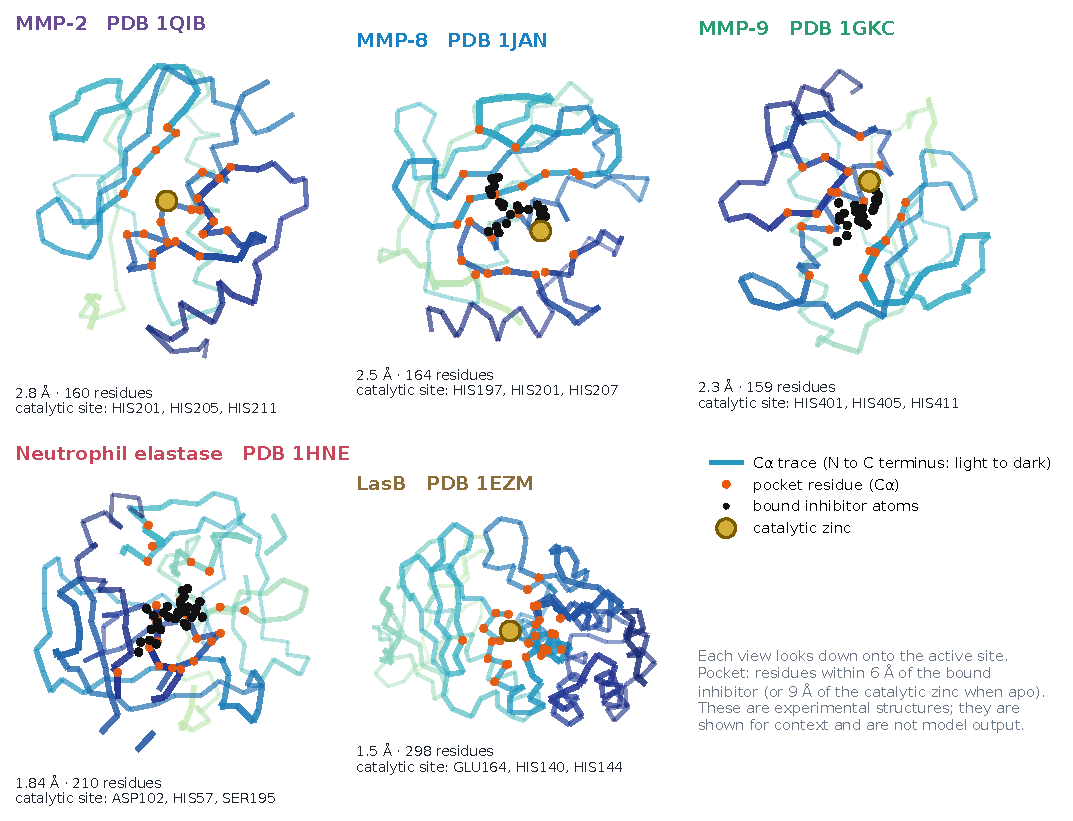
\includegraphics[width=\textwidth]{figures/F19_structures.pdf}
\caption{C$\alpha$ traces of the five structures, each oriented to look at the active site (depth-cued; N to C terminus from light to dark). Orange: pocket residues; gold: catalytic zinc; black: bound inhibitor atoms. These are experimental structures shown for context; they are not model output. MMP-9 is shown from an active catalytic-domain entry, not the pro-form, whose prodomain occupies the cleft.}
\label{fig:struct}
\end{figure}

\subsection{Held-out measured kinetics}
\label{sec:kval}
Kridel et al.\ (2001, their Table~II) measured $\kcat/\Km$ for MMP-9 on eleven synthetic peptides and found no detectable activity on a twelfth (C11). None of these peptides is in the training data after the removal of four coinciding windows (Section~\ref{sec:eval}). We score each as a gapped window (Table~\ref{tab:kscores}) and rank-correlate with $\log_{10}\kcat/\Km$.

\begin{table}[!htbp]
\centering\small\begin{tabular}{@{}llrrrr@{}}\toprule
Peptide & Window (P4--P4$'$) & Positions & MMP-9 $k_\mathrm{cat}/K_m$ (M$^{-1}$s$^{-1}$) & LR logit & PSSM \\\midrule
C15 & \texttt{GPRQITA-} & 7 & 188{,}000 & +2.07 & +5.41 \\
A11 & \texttt{IPRTLTA-} & 7 & 67{,}500 & +1.30 & +3.67 \\
A6 & \texttt{GPRAVSTT} & 8 & 61{,}000 & +1.24 & +4.20 \\
A11m1 & \texttt{IPRRLTA-} & 7 & 160{,}000 & +2.43 & +5.66 \\
A11m2 & \texttt{IPRTATA-} & 7 & 2{,}000 & +1.15 & +2.35 \\
A10 & \texttt{GPLFYSVT} & 8 & 25{,}600 & +0.33 & +2.70 \\
B1 & \texttt{QPHYLTTA} & 8 & 8{,}800 & +0.81 & +3.10 \\
A18 & \texttt{RPAKSTA-} & 7 & 5{,}800 & +1.28 & +4.96 \\
A7 & \texttt{--SGLKAL} & 6 & 12{,}400 & +0.77 & +3.08 \\
A19 & \texttt{GSRYLTA-} & 7 & 13{,}200 & +0.74 & +3.02 \\
A16 & \texttt{SGRRLLSR} & 8 & 1{,}200 & +0.68 & +0.78 \\
C11 & \texttt{SGRRLIHH} & 8 & not detected & +0.30 & +2.47 \\
\bottomrule\end{tabular}

\caption{Validation peptides (Kridel et al., 2001, Table II) as scored P4--P4$'$ windows, with measured MMP-9 $\kcat/\Km$ and model scores from the MMP-9 model retrained without coinciding windows. Positions: number of known positions out of eight.}
\label{tab:kscores}
\end{table}

\begin{table}[!htbp]
\centering\small\begin{tabular}{@{}llccc@{}}\toprule
Score & Set & Spearman $\rho$ & 95\% bootstrap CI & Permutation $p$ \\\midrule
Logistic regression & n = 11 measured & 0.58 & [-0.23, 0.93] & 0.068 \\
Logistic regression & n = 12 (C11 ranked lowest) & 0.68 & [0.02, 0.96] & 0.017 \\
PSSM & n = 11 measured & 0.70 & [-0.00, 0.96] & 0.020 \\
PSSM & n = 12 (C11 ranked lowest) & 0.75 & [0.18, 0.93] & 0.006 \\
Standardised mean & n = 11 measured & 0.57 & [-0.21, 0.90] & 0.074 \\
Standardised mean & n = 12 (C11 ranked lowest) & 0.66 & [0.06, 0.91] & 0.021 \\
\bottomrule\end{tabular}

\caption{Rank association between model score and measured MMP-9 $\kcat/\Km$. The permutation $p$-value is two-sided; intervals are bootstrap over peptides. The last rows include C11 (no activity detected) ranked below every measured peptide.}
\label{tab:kspear}
\end{table}

The association is positive for every scorer and every set (Table~\ref{tab:kspear}; Figure~\ref{fig:kval}). For the PSSM it is $\rho=\rhoNElevenPSSM$ on the eleven measured peptides (permutation $p=\rhoPNElevenPSSM$; $95\%$ interval $[\rhoLoNElevenPSSM,\rhoHiNElevenPSSM]$); for the logistic regression $\rho=\rhoNElevenLR$ ($p=\rhoPNElevenLR$). The intervals are wide and, for the logistic regression on $n=11$, include zero. With $n=11$ and a set that was itself selected for high activity, this is evidence of a positive association, not of accurate rate prediction, and the six tests are not corrected for multiplicity. By the logistic regression the three highest-scored peptides (A11m1, C15, A11) are the three most active; its largest miss is A10 ($25{,}600$~M$^{-1}$s$^{-1}$, the fifth most active), which it scores second-lowest. The PSSM scores the least active measured peptide (A16) lowest, but ranks A18 ($5{,}800$) third, its largest miss.

\begin{figure}[!htbp]
\centering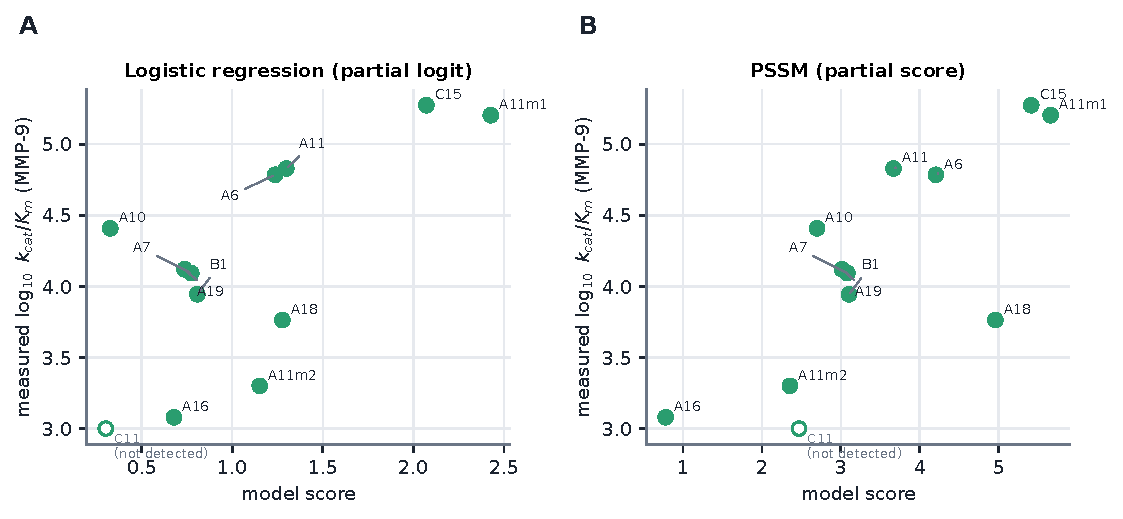
\includegraphics[width=\textwidth]{figures/F15_kridel_validation.pdf}
\caption{Model score against measured MMP-9 $\log_{10}\kcat/\Km$. Open marker: C11, no activity detected (plotted at the floor of the axis).}
\label{fig:kval}
\end{figure}

\subsubsection{Matched point mutants}
Two peptides are single-substitution mutants of A11 (SGKIPRT$\downarrow$LTA): A11m1 replaces Thr with Arg at $\pos{1}$; A11m2 replaces Leu with Ala at $\prm{1}$. Because the background is identical, they isolate one substitution each (Table~\ref{tab:kmut}). The model predicts the correct direction for both and roughly the correct size for the first ($+\mutOneLR$ bits from the logistic regression and $+\mutOnePSSM$ from the PSSM against a measured $+\mutOneMeasured$~log$_2$ units). For the second it predicts a decrease but underestimates it badly: $\mutTwoLR$ bits (logistic regression) and $\mutTwoPSSM$ bits (PSSM) against a measured $\mutTwoMeasured$. Large kinetic effects of a single key residue are compressed by a model trained to distinguish cleaved from uncleaved sites rather than fast from slow.

\begin{table}[!htbp]
\centering\small\begin{tabular}{@{}llccc@{}}\toprule
Pair & Substitution & Measured fold change (log$_2$) & LR $\Delta$ (bits) & PSSM $\Delta$ (bits) \\\midrule
A11$\to$A11m1 & T7R at P1 (Thr to Arg) & 2.37$\times$ (+1.25) & +1.63 & +1.99 \\
A11$\to$A11m2 & L8A at P1' (Leu to Ala) & 0.03$\times$ (-5.08) & -0.21 & -1.31 \\
\bottomrule\end{tabular}

\caption{Model change in score for the two matched mutants of A11, compared with the measured change in $\kcat/\Km$.}
\label{tab:kmut}
\end{table}

\section{Application to sensor design}
\label{sec:design}

\subsection{An alignment error in the design analysis, and its consequence}
The Task~8 design analysis defines candidate sensor cores as short motifs and scores them as eight-residue windows. Three of the four cores, PRSLSGLK, PLGLAGQS and PLGVALAA, are motifs whose scissile bond lies after the \emph{third} residue (Pro-Arg-Ser$\downarrow$Leu, Pro-Leu-Gly$\downarrow$Leu; $\pos{3}=\mathrm{Pro}$ and $\prm{1}=\mathrm{Leu}$, matching the consensus of Kridel et al.). Read as a P4--P4$'$ window, whose bond is after the fourth character, every residue is shifted one position from its intended subsite: for PRSLSGLK the window has $\pos{2}=\mathrm{S}$ and $\prm{1}=\mathrm{S}$ instead of $\pos{2}=\mathrm{R}$ and $\prm{1}=\mathrm{L}$. The design plan itself states the intended features as ``P2 = Arg, P1$'$ = Leu, P2$'$ = Ser'', which the shifted window does not encode.

The model responded correctly to the wrong input: PRSLSGLK scored at the $7$th percentile for MMP-9. Scored as the gapped window \texttt{-PRSLSGL} with the bond after the third residue, it scores at the $100$th percentile (and at the top for MMP-2 and MMP-8, Table~\ref{tab:cand}). The correction also changes a design conclusion. The $3\times3$ specificity matrix of the MMP-2/MMP-9/NE design analysis has condition number $61.7$ with the shifted windows (``poorly conditioned, pivot to a two-plex'' by the analysis's own rule) and $16.1$ with the corrected windows (``marginal''). The corrected matrix still shows that the MMP-2 and MMP-9 candidates are not separable by score, as the selectivity results of Section~\ref{sec:res-sel} predict.

\begin{table}[!htbp]
\centering\small\begin{tabular}{@{}llllcc@{}}\toprule
Candidate & Core & Scored window & Target & Margin (3-plex) & Pool percentile \\\midrule
Cand1 MMP9 & \texttt{PRSLSGLK} & \texttt{-PRSLSGL} & MMP-9 & -0.00 & 16 \\
Cand2 MMP2 & \texttt{PLGLAGQS} & \texttt{-PLGLAGQ} & MMP-2 & -0.00 & 0 \\
Cand4 NE & \texttt{AAPVSGIG} & \texttt{AAPVSGIG} & NE & +0.51 & 26 \\
Cand3 MMP2b & \texttt{PLGVALAA} & \texttt{-PLGVALA} & MMP-2 & -0.04 & 0 \\
\bottomrule\end{tabular}

\caption{Task~8 candidates scored in the MMP-2/MMP-9/NE panel with correctly aligned, gapped windows. ``Pool percentile'' is the percentile of the margin within the PSSM top-3 enumeration pool for the target (same gap pattern).}
\label{tab:design}
\end{table}

\subsection{Candidate landscape in the wound panel}
Figure~\ref{fig:cand} and Table~\ref{tab:cand} rank candidates in the five-protease wound panel (MMP-2, MMP-8, MMP-9, NE, LasB). The pool combines $150{,}000$ random windows with the PSSM top-3 enumerations of each target, filtered by the device constraints of the Task~8 design (no Cys or Trp, net charge $-1$ to $+2$, no Pro-Pro, core mass $600$--$1100$~Da). Three observations matter.

\begin{enumerate}
\item \textbf{The best-scoring sequences are model optima, not recommendations.} They are extreme points of a search over a random pool, far from any training window, and their scores extrapolate. They are hypotheses for wet-lab testing.
\item \textbf{The MMP-family reference cores have margin $\approx 0$.} The corrected MMP-9 cores (IPRTLTA$-$ and $-$PRSLSGL) score at the top for MMP-2, MMP-8 and MMP-9 alike, so no selectivity among MMPs is predicted. (Kridel et al.\ found A11 to be $2.9$-fold and $9.6$-fold more active on MMP-9 than on MMP-13 and MMP-7; neither is in our panel, so this cannot be tested here.)
\item \textbf{The panel changes the answer.} AAPVSGIG has margin $+0.51$ in the three-protease panel but $0.00$ in the wound panel, because the LasB model, trained largely on Gly/Ala/Pro-rich elastin sequence, scores it at the $99$th percentile. Whether LasB actually cleaves AAPV-type sites is not something these data can settle.
\end{enumerate}

\begin{figure}[!htbp]
\centering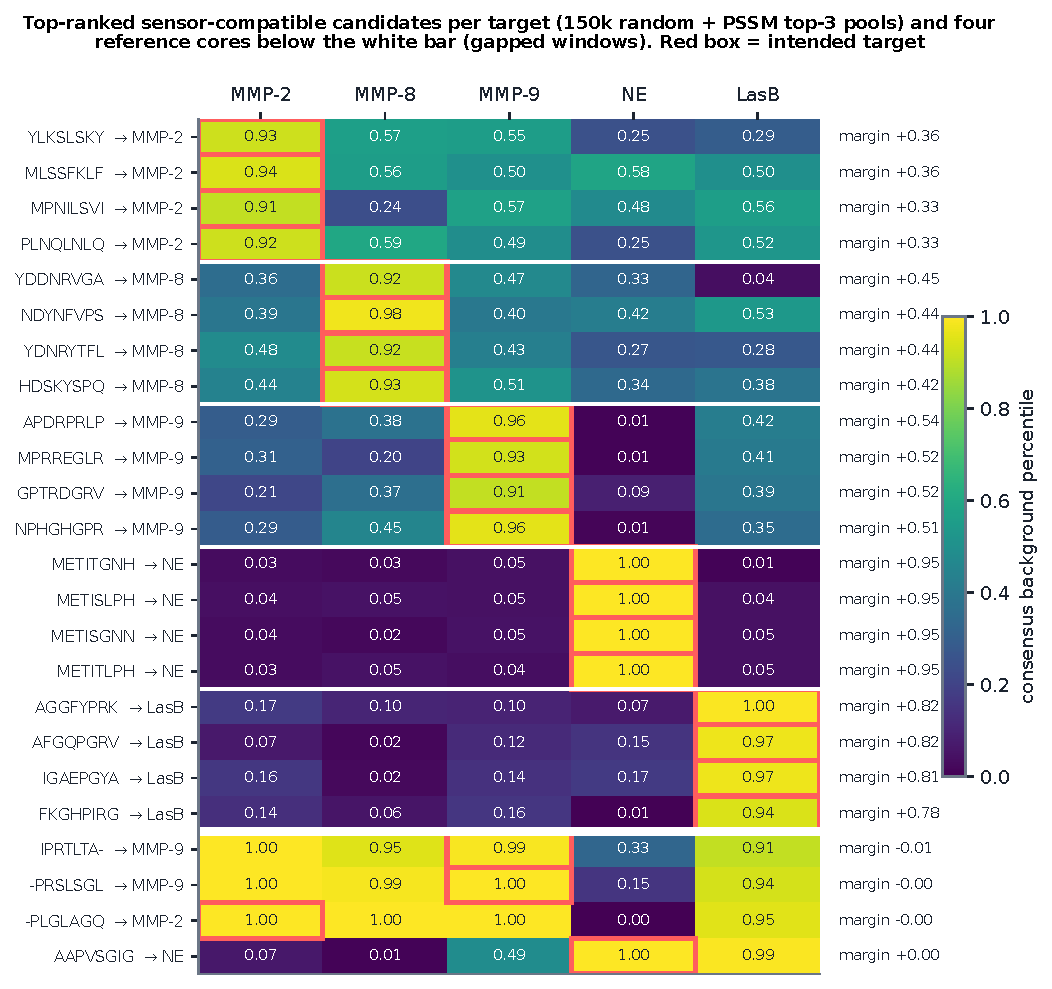
\includegraphics[width=0.85\textwidth]{figures/F17_candidate_landscape.pdf}
\caption{Consensus background percentiles of the four highest-margin sensor-compatible candidates for each target (above the white bar) and of four reference cores (below), across the five wound-panel proteases. Red boxes mark the intended target; margins are listed on the right. Reference cores are scored as gapped windows.}
\label{fig:cand}
\end{figure}

\begin{table}[!htbp]
\centering\small\begin{tabular}{@{}llccccc c@{}}\toprule
Window & Target & MMP-2 & MMP-8 & MMP-9 & NE & LasB & Margin \\\midrule
\texttt{YLKSLSKY} & MMP-2 & 0.93 & 0.57 & 0.55 & 0.25 & 0.29 & +0.36 \\
\texttt{MLSSFKLF} & MMP-2 & 0.94 & 0.56 & 0.50 & 0.58 & 0.50 & +0.36 \\
\texttt{MPNILSVI} & MMP-2 & 0.91 & 0.24 & 0.57 & 0.48 & 0.56 & +0.33 \\
\texttt{PLNQLNLQ} & MMP-2 & 0.92 & 0.59 & 0.49 & 0.25 & 0.52 & +0.33 \\
\texttt{YDDNRVGA} & MMP-8 & 0.36 & 0.92 & 0.47 & 0.33 & 0.04 & +0.45 \\
\texttt{NDYNFVPS} & MMP-8 & 0.39 & 0.98 & 0.40 & 0.42 & 0.53 & +0.44 \\
\texttt{YDNRYTFL} & MMP-8 & 0.48 & 0.92 & 0.43 & 0.27 & 0.28 & +0.44 \\
\texttt{HDSKYSPQ} & MMP-8 & 0.44 & 0.93 & 0.51 & 0.34 & 0.38 & +0.42 \\
\texttt{APDRPRLP} & MMP-9 & 0.29 & 0.38 & 0.96 & 0.01 & 0.42 & +0.54 \\
\texttt{MPRREGLR} & MMP-9 & 0.31 & 0.20 & 0.93 & 0.01 & 0.41 & +0.52 \\
\texttt{GPTRDGRV} & MMP-9 & 0.21 & 0.37 & 0.91 & 0.09 & 0.39 & +0.52 \\
\texttt{NPHGHGPR} & MMP-9 & 0.29 & 0.45 & 0.96 & 0.01 & 0.35 & +0.51 \\
\texttt{METITGNH} & Neutrophil elastase & 0.03 & 0.03 & 0.05 & 1.00 & 0.01 & +0.95 \\
\texttt{METISLPH} & Neutrophil elastase & 0.04 & 0.05 & 0.05 & 1.00 & 0.04 & +0.95 \\
\texttt{METISGNN} & Neutrophil elastase & 0.04 & 0.02 & 0.05 & 1.00 & 0.05 & +0.95 \\
\texttt{METITLPH} & Neutrophil elastase & 0.03 & 0.05 & 0.04 & 1.00 & 0.05 & +0.95 \\
\texttt{AGGFYPRK} & LasB & 0.17 & 0.10 & 0.10 & 0.07 & 1.00 & +0.82 \\
\texttt{AFGQPGRV} & LasB & 0.07 & 0.02 & 0.12 & 0.15 & 0.97 & +0.82 \\
\texttt{IGAEPGYA} & LasB & 0.16 & 0.02 & 0.14 & 0.17 & 0.97 & +0.81 \\
\texttt{FKGHPIRG} & LasB & 0.14 & 0.06 & 0.16 & 0.01 & 0.94 & +0.78 \\
\midrule
\texttt{IPRTLTA-} & MMP-9 & 1.00 & 0.95 & 0.99 & 0.33 & 0.91 & -0.01 \\
\texttt{-PRSLSGL} & MMP-9 & 1.00 & 0.99 & 1.00 & 0.15 & 0.94 & -0.00 \\
\texttt{-PLGLAGQ} & MMP-2 & 1.00 & 1.00 & 1.00 & 0.00 & 0.95 & -0.00 \\
\texttt{AAPVSGIG} & Neutrophil elastase & 0.07 & 0.01 & 0.49 & 1.00 & 0.99 & +0.00 \\
\bottomrule\end{tabular}

\caption{Consensus percentiles and specificity margin for the candidates of Figure~\ref{fig:cand}.}
\label{tab:cand}
\end{table}

\subsection{What each position contributes}
The scan in Figure~\ref{fig:scan} scores every single-residue substitution of IPRTLTA$-$ (the A11 core). Panel~(a) shows the change in the MMP-9 logistic-regression log-odds, which does not saturate; panel~(b) shows the change in specificity margin, which is near zero for most substitutions because the wild-type is already at the top of the MMP percentile scale. Substitutions at $\pos{3}$ are the most damaging (any replacement of Pro costs roughly $1$ to $2.5$ log-odds units), a change of Thr to Arg or Lys at $\pos{1}$ raises the score (consistent with the measured effect of A11m1), and $\prm{1}$ is comparatively tolerant in this model, which is the same underestimation seen for A11m2.

\begin{figure}[!htbp]
\centering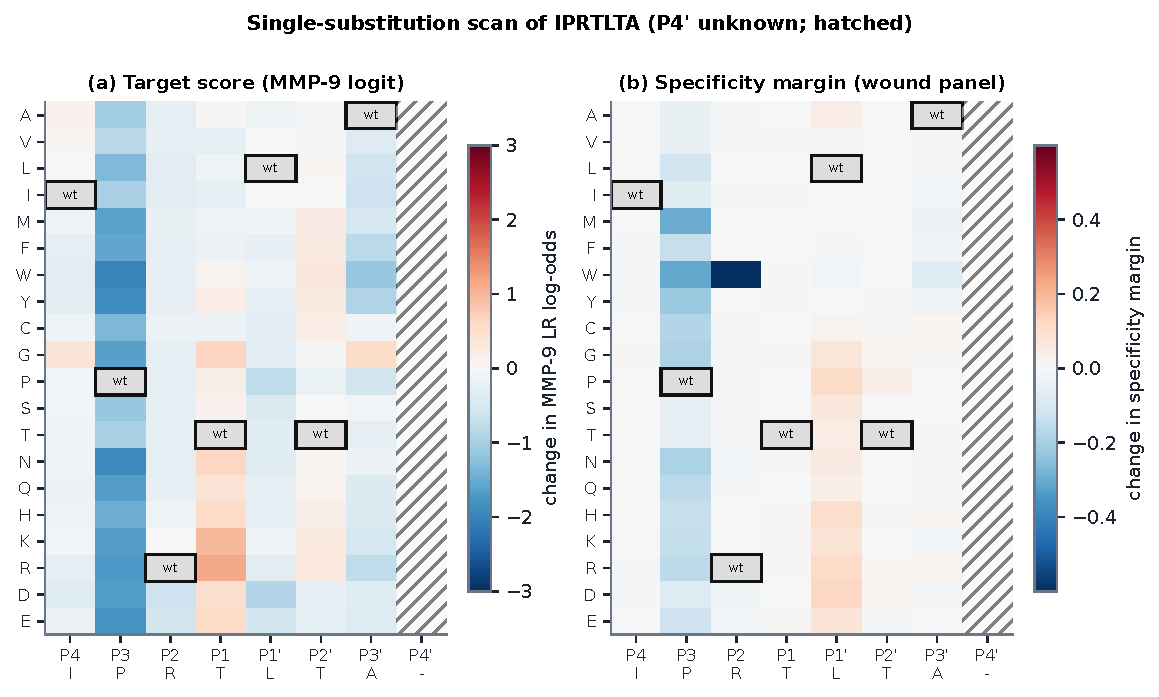
\includegraphics[width=\textwidth]{figures/F18_mutation_scan.pdf}
\caption{Single-substitution scan of the A11 core. \textbf{(a)} Change in MMP-9 logistic-regression log-odds. \textbf{(b)} Change in specificity margin in the wound panel.}
\label{fig:scan}
\end{figure}

\section{Limitations and threats to validity}
\label{sec:limits}

Each item states the limitation, the evidence for it where we have any, and what it means for use of the tool.

\begin{enumerate}
\item \textbf{Labels are positive--unlabelled.} No window is confirmed uncleaved, so every AUROC is compressed toward $0.5$ by an unknown contamination (Eq.~\ref{eq:contam-main}). \emph{Implication:} reported AUROCs are conservative for detection, and low cross-protease AUROCs partly reflect real promiscuity (Section~\ref{sec:contam}).
\item \textbf{The window is the whole input.} Only P4--P4$'$ is modelled. Distal exosite contacts, secondary structure, the flanking construct (linker, anchor, label), pH, ionic strength and temperature are all absent. \emph{Implication:} a sensor construct may behave differently from its core.
\item \textbf{Cleavage is binary, not a rate.} The models rank windows by resemblance to observed sites. External kinetics correlate positively but modestly ($n=11$), large single-residue kinetic effects are underestimated (A11m2), and no rate constant is predicted. \emph{Implication:} use scores to shortlist, then measure $\kcat/\Km$.
\item \textbf{Selectivity within the MMP family is weak.} Held-out AUROC between MMP substrate sets is $0.53$--$0.72$, and MMP-family cores reach margin $\approx0$. \emph{Implication:} do not rely on sequence alone to distinguish MMP-2, -8, -9 and -14.
\item \textbf{The LasB model is confounded by its source.} $97$ of $128$ positives ($76\%$) are windows from one protein, elastin, and composition alone separates them from background as well as the full model does ($0.886$ versus $0.877$). \emph{Implication:} the LasB score behaves as an elastin-likeness score; it inflates competitor percentiles for Gly/Ala/Pro-rich peptides (as for AAPVSGIG) and should not be read as LasB specificity.
\item \textbf{The faecal group is heterogeneous.} It pools three unrelated digestive proteases from three species and its data are dominated by a Lys/Arg preference at $\pos{1}$. \emph{Implication:} it is a distinctness control, not a model of a single enzyme.
\item \textbf{Source biases.} MEROPS mixes physiological and synthetic substrates and is curated by literature attention; PICS libraries are generated with trypsin or GluC, constraining composition at peptide ends; the NE model ranks Cys among its top residues at several positions, possibly reflecting cysteine-rich source proteins. \emph{Implication:} learned specificity is that of the sampled substrates, not of the enzyme in the abstract.
\item \textbf{Percentile scale resolution.} Percentiles are interpolated from a $1{,}001$-point grid, so the top of the scale saturates at $10^{-3}$ and margins near zero can hide real score differences among strong candidates (Figure~\ref{fig:scan}). \emph{Implication:} for fine ranking among strong candidates use the raw logit and PSSM scores alongside the margin.
\item \textbf{The consensus and margin are heuristics.} The harmonic-mean combination and the max-competitor margin are reasoned but not tuned or validated against a selectivity ground truth. \emph{Implication:} treat margins as ordinal.
\item \textbf{Extrapolation.} Optimised candidates lie far from the training distribution, where neither the models nor their percentile scales have been checked. \emph{Implication:} candidate lists are hypotheses.
\item \textbf{Small external validation.} Eleven peptides, all phage-selected for MMP-9 activity, six uncorrected tests, and no MMP-13/MMP-7 models with which to test the reported selectivity. \emph{Implication:} the external result supports direction, not magnitude.
\item \textbf{No prospective wet-lab test yet.} The strongest test of the tool is a blind prediction of measured relative activity of new peptides across the panel. It has not been done.
\end{enumerate}

\section{Reproducibility}
\label{sec:repro}

Everything in this report is regenerated from the repository by the following commands (Python $\ge3.10$; scikit-learn, NumPy, pandas, SciPy, LightGBM for the model comparison; a TeX distribution for the document):
\begin{Verbatim}[fontsize=\small,frame=single,rulecolor=\color{ink!40}]
python -m spred build-data              # positives from source files
python -m spred train                   # cross-validation, nested tuning, final models
python scripts/methodology.py           # models, learning curves, negative designs
python scripts/leakage_check.py         # random vs cluster folds
python scripts/representation_analysis.py
python scripts/coefficient_stability.py
python scripts/validation.py            # external validation (Kridel et al.)
python scripts/prepare_structures.py    # structure facts from coordinates
python report/figs_*.py; python report/make_tables.py
python -m pytest tests -q               # 28 tests
\end{Verbatim}
Random seeds are fixed ($42$ throughout; the background null uses seed $43$). Each trained model records its training-data fingerprint, cross-validated metrics, and selected regularisation. Reference tables (VHSE, BLOSUM62, Swiss-Prot composition) are archived with their provenance under \texttt{references/} and are compared with the code's tables by unit tests. The trained models are plain JSON and are embedded in the accompanying browser tool, which is tested for numerical agreement with the Python package.

\appendix
\section{Derivations}
\label{app:deriv}

\subsection{AUROC equals the Mann--Whitney probability}
Let $S^{+}$ and $S^{-}$ be independent scores of a random positive and a random negative, with densities $f_1$ and $f_0$ and survival functions $\bar F_1(\tau)=\Prob(S^{+}>\tau)$, $\bar F_0(\tau)=\Prob(S^{-}>\tau)$. The ROC curve traces $(\mathrm{FPR},\mathrm{TPR})=(\bar F_0(\tau),\bar F_1(\tau))$ as $\tau$ decreases from $+\infty$ to $-\infty$, so, since $d\bar F_0(\tau)=-f_0(\tau)\,d\tau$,
\begin{equation}
\mathrm{AUROC}=\int \mathrm{TPR}\;d\mathrm{FPR}=\int_{-\infty}^{\infty}\bar F_1(\tau)\,f_0(\tau)\,d\tau=\Prob(S^{+}>S^{-}).
\end{equation}
With ties, $\mathrm{AUROC}=\Prob(S^{+}>S^{-})+\tfrac12\Prob(S^{+}=S^{-})$. Its empirical estimator is $U/(n_+n_-)$, where $U$ is the Mann--Whitney statistic. This shows AUROC is threshold-free, invariant under any strictly increasing transformation of the score, and unaffected by the class ratio, which is why it is comparable across our $1{:}3$ training sets and across models on different scales.

\subsection{Label contamination}
Suppose the negatives are a mixture: with probability $\pi$ a ``negative'' is a hidden positive drawn from the same distribution as the labelled positives, and with probability $1-\pi$ a true negative. For a fixed continuous scorer,
\begin{align}
\mathrm{AUROC}_{\text{measured}}&=\Prob(S^{+}>S_{\text{neg}})=(1-\pi)\Prob(S^{+}>S^{-}_{\text{true}})+\pi\,\Prob(S^{+}>S^{+\prime})\notag\\
&=(1-\pi)\,\mathrm{AUROC}_{\text{true}}+\tfrac12\pi,
\label{eq:contam}
\end{align}
since two independent draws from the same continuous distribution are ordered either way with probability $\tfrac12$. The measured value therefore lies between $0.5$ and $\mathrm{AUROC}_{\text{true}}$ (whenever $\mathrm{AUROC}_{\text{true}}>0.5$) and is at most $1-\pi/2$ even for a perfect scorer. Contamination can only lower AUROC.

\subsection{Exact near-duplicate clustering by pigeonhole}
Partition the eight positions into blocks $B_1=\{1,2,3\}$, $B_2=\{4,5,6\}$, $B_3=\{7,8\}$. If two windows differ at no more than two positions, those positions occupy at most two of the three blocks, so at least one block contains no mismatch and the two windows are identical on that block. Hence every pair at Hamming distance $\le2$ appears together in at least one bucket of windows keyed by the content of a single block. Comparing only windows within a bucket therefore finds \emph{all} such pairs; the connected components are found with union--find. The result is exact, and its cost is governed by bucket sizes rather than by $n^2$. The implementation is tested against brute-force comparison.

\subsection{Convexity of the logistic objective}
Write $m_i=\bm\beta^{\top}\bm z_i+b$, $p_i=\sigma(m_i)$, $\tilde y_i=2y_i-1$. Since $\frac{d}{dm}\log(1+e^{-\tilde ym})=-\tilde y\,\sigma(-\tilde ym)$, the gradient of Eq.~\eqref{eq:lr} is
\begin{equation}
\nabla_{\bm\beta}\mathcal{L}=\bm\beta-C\sum_i\omega_{y_i}\tilde y_i\,\sigma(-\tilde y_im_i)\,\bm z_i,\qquad
\partial_b\mathcal{L}=-C\sum_i\omega_{y_i}\tilde y_i\,\sigma(-\tilde y_im_i).
\end{equation}
The Hessian with respect to $(\bm\beta,b)$ is $\mathrm{diag}(\bm I,0)+C\sum_i\omega_{y_i}p_i(1-p_i)\tilde{\bm z}_i\tilde{\bm z}_i^{\top}$ with $\tilde{\bm z}_i=[\bm z_i;1]$. For a direction $\bm v=(\bm v_\beta,v_b)$, $\bm v^{\top}H\bm v=\|\bm v_\beta\|^2+C\sum_i\omega_{y_i}p_i(1-p_i)(\bm z_i^{\top}\bm v_\beta+v_b)^2\ge0$, and it vanishes only if $\bm v_\beta=\bm 0$ and then $v_b^2\sum_i\omega_{y_i}p_i(1-p_i)=0$, i.e.\ $v_b=0$. The Hessian is therefore positive definite, the objective is strictly convex, and the minimiser is unique.

\subsection{Percentile scores are comparable across models}
Let $S$ have a continuous distribution function $F$. Then $\Prob(F(S)\le u)=\Prob(S\le F^{-1}(u))=u$, so $F(S)\sim\mathrm{Uniform}(0,1)$. For each protease we set $F$ to the null distribution of its own score over random windows, so under the null every protease's percentile is uniform on $[0,1]$: a percentile of $0.99$ means the same thing (exceeded by $1\%$ of random windows) for every model, regardless of how its raw score is scaled. For any strictly increasing $g$, $F_{g(S)}(g(s))=F_S(s)$, so the percentile does not depend on the monotone form of the score (logit versus probability, for instance). The harmonic mean $H(a,b)=2ab/(a+b)$ satisfies $\min(a,b)\le H(a,b)\le\tfrac12(a+b)$ and equals $1$ only when $a=b=1$, so it is high only when both percentiles are.

\subsection{Unknown positions}
Let the logit be $L(\bm z)=b+\sum_i\bm\beta_i^{\top}\bm z_i$. If the block $\bm z_j$ of an unknown position is random with mean $\bm 0$ (its standardised training mean) and independent of the rest, then $\E[L]=b+\sum_{i\ne j}\bm\beta_i^{\top}\bm z_i$, which is $L$ with $\bm z_j$ set to $\bm 0$. This is exact for the logit and does not hold for the probability $\sigma(L)$, which is why the imputation is applied to the logit. For the PSSM, the expected contribution of position $j$ under the background $g$ is
\begin{equation}
\sum_a g(a)\log_2\frac{p_j(a)}{g(a)}=-D_{\mathrm{KL}}(g\,\|\,p_j)\le0,
\end{equation}
so an unknown position lowers the score by an amount that grows with how informative that position is.

\subsection{Coverage of the VHSE subspace}
Let $\Phi\in\R^{20\times8}$ hold the VHSE descriptors and $\bm 1$ a column of ones; $\operatorname{rank}[\Phi,\bm1]=9$ (numerically). For a position with centred log-odds vector $\bm v\in\R^{20}$ and $P$ the orthogonal projector onto $\operatorname{span}[\Phi,\bm1]$, the fraction of its variance expressible by the encoding is $R^2=1-\|(\bm I-P)\bm v\|^2/\|\bm v\|^2$; Table~\ref{tab:controls} reports the average over positions weighted by $\|\bm v\|^2$. The unexpressible remainder is the encoding's approximation bias for that protease.

\section{Audit of the previous implementation}
\label{app:audit}

The models in this report replace an earlier implementation that had grown through several generations of scripts and model files. Before rebuilding, each element was tested with code. The table lists what was found and what was done; the evidence is in the repository history (the audit was run at commit \texttt{68e3dc2}; its outputs are kept in \texttt{results/legacy\_audit/}).

\begin{table}[!htbp]
\centering\footnotesize
\begin{tabular}{@{}p{0.2\textwidth}p{0.42\textwidth}p{0.3\textwidth}@{}}\toprule
Element & Finding & Action \\\midrule
VHSE descriptor table & $35$ of $160$ values differed from the archived published table (several with opposite sign); glycine was set to an all-zero ``reference'' vector, which is false; descriptor labels (H-bond donor, H-bond acceptor, charge) contradict the source's hydrophobic/steric/electronic definition; the citation named the wrong journal. Correcting the table changed random-fold AUROC by $-0.006$ to $+0.012$. & Table regenerated from the archived file and unit-tested against it; labels and citation corrected. \\
Swiss-Prot background & Two different frequency tables were in use (a residue frequency differed by up to $0.0049$ between them). & One table from release 2026\_03, imported everywhere. \\
Grouped cross-validation & Reported as $0.5$ for every protease. The groups were the labels ``positive / cross / background'', so every held-out group contained a single class and was skipped, and the function returned a hard-coded fallback. & Replaced by cluster-aware folds and cluster-bootstrap intervals. \\
PSSM performance & Scored on the positives used to build the PSSM. In-sample versus out-of-fold AUROC: LasB $0.977$ versus $0.779$, NE $0.883$ versus $0.829$, MMP-8 $0.875$ versus $0.849$, MMP-9 $0.816$ versus $0.790$. & PSSM refit and scored out-of-fold in every fold. \\
Selectivity index & The ratio $p_t/\max p_j$ compared probabilities from models whose mean score on random windows ranged $0.106$ to $0.328$; the median index for the top $1\%$ of MMP-9 candidates was $0.975$. & Percentile scale and margin (Section~\ref{sec:null}). \\
LasB training data & $92$ ``positives'' were generated by a rule (every Ala$|$Ala, Val$|$Ala, Ala$|$Gly and Gly$|$Ala bond in a hard-coded elastin string) and attributed to a paper not held; $14$ more were typed by hand; four windows tagged as MEROPS were absent from the MEROPS file. None is a measured cleavage site. & Removed. LasB uses the $31$ windows present in MEROPS and $97$ from Yang et al. \\
Elastin table (Yang et al.) & Typed by hand from the PDF: four of $75$ rows did not appear in the source (a typo and missing residues). & Re-extracted directly from the PDF; all $75$ rows verified against UniProt P04985. \\
Kinetic table & The competing enzymes were labelled MMP-1/MMP-2; the source table gives MMP-13 and MMP-7. One measured non-substrate (C11) was omitted. & Re-extracted from the paper's Table~II. \\
Report and code drift & Positive counts in the old report (MMP-14 $129$, MMP-8 $96$, MMP-9 $341$) no longer matched the data ($717$, $698$, $783$ after PICS integration); a unit test asserted the false glycine claim; oversampling was applied before cross-validation (never triggered at the $1{:}3$ ratio, but a leak if it were). & Report rewritten; test corrected; oversampling removed. \\
Model sprawl & Separate model files and scripts per experiment (panels A and B, ``v2'', ``v3'', LasB) overwriting one another's files. & One model per protease; panels are a scoring-time choice. \\
Design analysis & The AUROC figure used typed-in values (MMP-8 with $427$ positives against $698$ actual, in-sample PSSM AUROCs); three candidate cores were scored one residue out of register (Section~\ref{sec:design}). & Figures read the result files; candidates scored as gapped, correctly aligned windows. \\\bottomrule
\end{tabular}
\caption{Defects in the earlier implementation, found by executed checks, and their resolution.}
\end{table}

\section{Supplementary tables}

\begin{table}[!htbp]
\centering\small\begin{tabular}{@{}lcccccccc@{}}\toprule
Protease & P4 & P3 & P2 & P1 & P1$'$ & P2$'$ & P3$'$ & P4$'$ \\\midrule
MMP-2 & \texttt{PQG} & \texttt{PVI} & \texttt{ASQ} & \texttt{NGA} & \texttt{LIM} & \texttt{VQK} & \texttt{GSA} & \texttt{PDQ} \\
MMP-8 & \texttt{GKH} & \texttt{PAV} & \texttt{QCY} & \texttt{NKE} & \texttt{LCY} & \texttt{VHM} & \texttt{GAH} & \texttt{PAH} \\
MMP-9 & \texttt{GPK} & \texttt{PAV} & \texttt{APQ} & \texttt{GKR} & \texttt{LIQ} & \texttt{HQY} & \texttt{GAS} & \texttt{PHG} \\
MMP-14 & \texttt{HNG} & \texttt{PCV} & \texttt{CAQ} & \texttt{NGH} & \texttt{LCI} & \texttt{MVQ} & \texttt{HAV} & \texttt{PHK} \\
Neutrophil elastase & \texttt{PCM} & \texttt{QET} & \texttt{PCT} & \texttt{VIT} & \texttt{TMS} & \texttt{WLG} & \texttt{PCN} & \texttt{PHN} \\
LasB & \texttt{GAV} & \texttt{GPA} & \texttt{GPA} & \texttt{GPA} & \texttt{GFV} & \texttt{GPA} & \texttt{GPV} & \texttt{GPV} \\
Faecal & \texttt{EQD} & \texttt{QFL} & \texttt{QPE} & \texttt{KRG} & \texttt{TVA} & \texttt{LQV} & \texttt{QEP} & \texttt{EQD} \\
\bottomrule\end{tabular}

\caption{Top three residues by PSSM log-odds at each position, per protease (best first).}
\label{tab:topres}
\end{table}

\section*{References}
\addcontentsline{toc}{section}{References}
\small
\begin{enumerate}[label={[\arabic*]},leftmargin=*,itemsep=0.25em]
\item Kridel SJ, Chen E, Kotra LP, Howard EW, Mobashery S, Smith JW (2001). Substrate hydrolysis by matrix metalloproteinase-9. \textit{J Biol Chem} 276(23):20572--20578. doi:10.1074/jbc.M100900200. \emph{(Full text held in the repository.)}
\item Nagase H, Woessner JF Jr (1999). Matrix metalloproteinases. \textit{J Biol Chem} 274(31):21491--21494. \emph{(Full text held; bibliographic details as printed in the file.)}
\item Trengove NJ, Stacey MC, MacAuley S, Bennett N, Gibson J, Burslem F, Murphy G, Schultz G (1999). Analysis of the acute and chronic wound environments: the role of proteases and their inhibitors. \textit{Wound Repair Regen} 7:442--452. \emph{(Full text held.)}
\item Eckhard U, Huesgen PF, Schilling O, Bellac CL, Butler GS, Cox JH, Dufour A, Goebeler V, Kappelhoff R, Keller UAD, Klein T, Lange PF, Marino G, Morrison CJ, Prudova A, Rodriguez D, Starr AE, Wang Y, Overall CM (2016). Active site specificity profiling of the matrix metalloproteinase family: proteomic identification of 4300 cleavage sites by nine MMPs explored with structural and synthetic peptide cleavage analyses. \textit{Matrix Biol} 49:37--60. doi:10.1016/j.matbio.2015.09.003. \emph{(Supplementary tables held and used as data.)}
\item Yang J, Zhao HL, Ran LY, Li CY, Zhang XY, Su HN, Shi M, Zhou BC, Chen XL, Zhang YZ (2015). Mechanistic insights into elastin degradation by pseudolysin, the major virulence factor of the opportunistic pathogen \emph{Pseudomonas aeruginosa}. \textit{Sci Rep} 5:9936. doi:10.1038/srep09936. \emph{(Supplementary data held and used as data.)}
\end{enumerate}

\subsection*{Method and data attributions (records verified; full text not held)}
\begin{enumerate}[label={[M\arabic*]},leftmargin=*,itemsep=0.2em]
\item Mei H, Liao ZH, Zhou Y, Li SZ (2005). A new set of amino acid descriptors and its application in peptide QSARs. \textit{Biopolymers} 80(6):775--786. doi:10.1002/bip.20296. Descriptor definition checked against the published abstract; values archived from the \texttt{peptides} package v0.5.0 (\texttt{references/}).
\item Henikoff S, Henikoff JG (1992). Amino acid substitution matrices from protein blocks. \textit{Proc Natl Acad Sci USA} 89:10915--10919. doi:10.1073/pnas.89.22.10915. Matrix values taken from Biopython 1.87 and compared with the code's table (identical).
\item MEROPS peptidase database, \texttt{Substrate\_search} and peptidase-unit records (identifiers and names used as given in the records).
\item UniProt Consortium. UniProtKB/Swiss-Prot release 2026\_03, amino-acid composition (Expasy release statistics, section 6.1, archived); sequence P04985 (bovine elastin).
\item RCSB Protein Data Bank entries 1GKC (Rowsell et al., 2002, \textit{J Mol Biol} 319:173), 1QIB, 1JAN, 1HNE, 1EZM; titles and resolutions as recorded by the PDB.
\item Software: scikit-learn (logistic regression, cross-validation), LightGBM (gradient boosting, comparison only), NumPy, pandas, SciPy, matplotlib, Biopython.
\end{enumerate}

\end{document}
